\section{Relle Zahlen}

\begin{definition}
	Eine Menge $A$ heißt \emph{abzählbar}, falls es eine surjektive Abbildung $\f{\naturalset}{A}$ gibt.
\end{definition}

\begin{definition}
	Die reellen Zahlen sind angeordnet, d.h. es gibt ein Prädikat $a > 0$ sodass
	\begin{enumerate}[noitemsep]
		\item $\forallinreal{a}$ gilt genau einer der Aussagen $a = 0, a < 0, -a < 0$
		\item $\forallinreal{a,b}$ mit $a > 0, b > 0$ gilt: $a + b > 0, a \cdot b > 0$
	\end{enumerate}
\end{definition}

\begin{definition}
	Folgende Mengen nennen wir Intervalle:
	\begin{align}
		(a,b) &:= \{ \inreal{x} \medspace | \medspace  a    < x    < b \} & \textnormal{offenes Intervall}       \\
		[a,b] &:= \{ \inreal{x} \medspace | \medspace  a \leq x \leq b \} & \textnormal{geschlossenes Intervall} \\
		(a,b] &:= \{ \inreal{x} \medspace | \medspace  a    < x \leq b \} & \textnormal{halboffenes Intervall}   \\
		[a,b) &:= \{ \inreal{x} \medspace | \medspace  a \leq x    < b \} & \textnormal{halboffenes Intervall}	
	\end{align}
\end{definition}

\begin{definition}
	Eine Menge $M \subseteq \realset$ heißt \emph{beschränkt}, wenn
	\begin{enumerate}[noitemsep]
		\item $\exists s_0 \in \realset : \forallin{a}{M} : a \leq s_0$; $s_0$ heißt \emph{Obere Schranke}
		\item Ist $s_0$ zusätzlich die kleinste obere Schranke, so heißt $s_0$ \emph{Supremum}
		\item $\exists s_0 \in \realset : \forallin{a}{M} : s_0 \leq a$; $s_0$ heißt \emph{Untere Schranke}
		\item Ist $s_0$ zusätzlich die größte untere Schranke, so heißt $s_0$ \emph{Infimum}
	\end{enumerate}
\end{definition}

\begin{satz}[Supremumsaxiom]
	Es gilt:
	\begin{enumerate}[noitemsep]
		\item Jede nichtleere nach oben beschränlte Menge $M \subseteq \realset$ besitzt ein Supremum, $sup(M) \in \realset$
		\item Jede nichtleere nach unten beschränlte Menge $M \subseteq \realset$ besitzt ein Infimum, $inf(M) \in \realset$
		\item $sup(M) \in M \rightarrow sup(M)$ heißt auch Maximum von $M$
		\item $inf(M) \in M \rightarrow inf(M)$ heißt auch Minimum von $M$
	\end{enumerate}
\end{satz}

\begin{satz}[Archimedizität]
	$\realset$ ist archimedisch, d.h. $\forallinreal{a} : \exists n \in \naturalset : a < n $. Jede relle Zahl besitzt also ein natürliches Supremum. Insbesondere gilt auch (offensichtlich, aber für Konvergenzbeweise hilfreich): $\frac{1}{n} < a$.
\end{satz}

\begin{satz}[Abschätzungen]
	Es gelten die folgenden Abschätzungen:
	
	\begin{enumerate}[noitemsep]
		\item \textbf{\emph{Dreiecksungleichung:}} $\forallinreal{x,y} : | x + y | \leq |x| + |y|$
		\item \textbf{\emph{Umgekehrte Dreiecksungleichung:}} 	$\forallinreal{x,y} : | x + y | \geq ||x| - |y||$
		\item \textbf{\emph{Cauchy-Schwarz-Ungleichung:}} 	$\forallinreal{x,y}^n : | \inner{x}{y}|^2 \leq ||x||^2 \cdot ||y||^2$
		\item \textbf{\emph{Abschätzen von Polynomen}} 	$ax^2 + bx + c \leq (a + b + c)x^2 $
		\item \textbf{\emph{Abschätzen der Wurzel:}} 	$\sqrt{ab} \leq \frac{a + b}{2}$
		\item \textbf{\emph{Bernoulli-Ungleichung:}} 	$(1+x)^n \geq 1 + nx$ für $x > -1$	
	\end{enumerate}
	
\end{satz}

\begin{satz}[Binomischer Lehrsatz]
	$\sum_{k=0}^{n} \binom{n}{k}a^k b^{n-k} = (a+b)^n$ 
\end{satz}

\section{Folgen}

\begin{definition}
	Eine Folge reeller Zahlen ist eine Abbildung $\naturalset \rightarrow \realset : n \rightarrow a_n$. $\sequencean$ beschreibt dabei die Folge, $a_n$ einen Folgenindex
\end{definition}


\begin{definition}
	Eine Folge $\sequencean$ konvergiert gegen $a \in \realset$ genau dann wenn \\ $\forall \epsilon > 0 : \exists n_0 \in \naturalset : \forall n \geq n_0 : | a_n - a | < \epsilon$, d.h. egal wie klein $\epsilon$, findet man eine Indexschranke $n_0$ sodass alle Folgeindices $a_n$ einen Abstand zu $a$ kleiner als $\epsilon$ haben. Wir schreiben $\liminfty{n} a_n = a$
\end{definition}

\begin{definition}
	Eine Folge $\sequencean$ divergiert, wenn sie nicht konvergiert. Sie konvergiert zusätzlich uneigentlich gegen
	\begin{enumerate}[noitemsep]
		\item $+ \infty$ genau dann wenn $\forall k > 0 : \exists n_0 \in \naturalset : \forall n \geq n_0 : a_n \geq k$, d.h. ab einen Index sind all $a_n \geq k$
		\item $- \infty$ genau dann wenn $\forall k > 0 : \exists n_0 \in \naturalset : \forall n \geq n_0 : a_n \leq -k$, d.h. ab einen Index sind all $a_n \leq -k$		
	\end{enumerate}
\end{definition}

\begin{definition}
	Eine Folge $\sequencean$ heißt \emph{beschränkt}, falls $\exists c > 0 : \forallin{n}{\naturalset} : a_n \leq c$
\end{definition}

\begin{satz}[Rechenregeln für Grenzwerte]
	Falls $\liminfty{n} a_n = a \in \realset$ sowie \\ $\liminfty{n} b_n = b \in \realset$, gilt:
	\begin{enumerate}[noitemsep]
		\item $\liminfty{n} (a_n \pm b_n) = \liminfty{n} a_n \pm \liminfty{n} b_n = a \pm b $
		\item $\liminfty{n} c \cdot a_n = c \cdot \liminfty{n} a_n = c \cdot a  $
		\item $\liminfty{n} a_nb_n = \liminfty{n} a_n \cdot \liminfty{n} b_n = ab  $
		\item $b \neq 0 \rightarrow\liminfty{n} \frac{a_n}{b_n} = \frac{\liminfty{n} a_n}{\liminfty{n} b_n} = \frac{a}{b} $
		\item $\liminfty{n} \sqrt{a_n} = \sqrt{a} $
		\item $\liminfty{n} |a_n| = |a| $
	\end{enumerate}
\end{satz}

\begin{satz}[Einschließungsregel]
	Es gelte $a_n \leq b_n \leq c_n$ für alle bis auf endlich viele $n$. Falls $\liminfty{n} a_n = \alpha$ und $\liminfty{n} c_n = \alpha $, dann ist auch $\liminfty{n} b_n = \alpha$.
\end{satz}

\begin{definition}[Monotone Folgen]
	Eine Folge $\sequencean$ heißt
	\begin{enumerate}[noitemsep]
		\item \emph{monoton fallend}, falls $a_n \geq a_{n+1}$ für alle $a_n$
		\item \emph{monoton steigend}, falls $a_n \leq a_{n+1}$ für alle $a_n$
		\item Gilt sogar $<$ bzw. $>$, so spricht man von \emph{strenger Monotonie}
	\end{enumerate}
\end{definition}

\begin{satz}[Monotonie und Konvergenz]
	Es gilt:
	\begin{enumerate}[noitemsep]
		\item $\sequencean$ monoton wachsend $\rightarrow \liminfty{n} a_n = sup(a_n)$
		\item $\sequencean$ monoton fallend $\rightarrow \liminfty{n} a_n = inf(a_n)$
		\item Jede beschränkte monotone Folge konvergiert
		\item Jede unbeschränkte monotone Folge konvergiert uneigentlich gegen $\pm \infty$
	\end{enumerate}
\end{satz}

\begin{definition}[Asymptotische Gleichheit]
	 $\sequencean$,  $\sequencebn$ heißen asymptotisch gleich, falls $\liminfty{n} \frac{a_n}{b_n} = 1$. Man schreibt: $a_n \backsimeq b_n$
\end{definition}

\section{Reihen}


\begin{definition}
	Zu einer Folge $\sequencean$ sei $(s_n)_{n \in \naturalset}$ mit $s_n := \sum_{k=0}^{n} a_k$ die Folge der Partialsummen. $\liminfty{n} s_n = \liminfty{n} \sum_{k=0}^{n} a_k = \serieskzeroinfty{a}$ heißt Werte der Reihe. Die Reihe konvergiert, wenn $(s_n)_{n \in \naturalset}$ konvergiert, sonst divergiert sie.
\end{definition}

\begin{satz}[Konvergenzkriterium]
	 $\serieskzeroinfty{a} $ konvergiert $\rightarrow \liminfty{k} a_k = 0$
\end{satz}

\begin{satz}[Majorantenkriterium]
	Es gilt:
	\begin{enumerate}[noitemsep]
		\item Findet man zur Reihe	$\serieskzeroinfty{a}$ eine Reihe $\serieskzeroinfty{b} $ sodass $b_k \geq |a_k|$, dann gilt: $\serieskzeroinfty{b}$ konvergiert $\rightarrow \sum_{k=0}^{\infty} a_k $ konvergiert. $\serieskzeroinfty{b} $ heißt Majorante
		\item Findet man zur Reihe	$\serieskzeroinfty{a}$ eine Reihe $\serieskzeroinfty{b} $ sodass $|b_k| \leq a_k$, dann gilt: $\serieskzeroinfty{b}$ divergiert $\rightarrow \sum_{k=0}^{\infty} a_k $ divergiert. $\serieskzeroinfty{b} $ heißt Minorante	
	\end{enumerate}
\end{satz}

\begin{satz}[Konvergenzkriterium]
	Sind die Folgen $\sequencean$ und $\sequencebn$ asymptotisch gleich, dann sind $\serieskzeroinfty{a}$ und $\serieskzeroinfty{b}$ entweder beide konvergent oder beide divergent.
\end{satz}

\begin{satz}[Quotientenkriterium]
	Sei $a_k \neq 0$ bis auf endlich viele $k$. Dann gilt:
	\begin{equation}
		\liminfty{k} | \frac{a_{k + 1}}{a_k} | = 
		\begin{cases}
		< 1 & \rightarrow \sum_{k=0}^{\infty} a_k \medspace \textnormal{ist konvergent} \\ 
		> 1 & \rightarrow \sum_{k=0}^{\infty} a_k \medspace \textnormal{ist divergent}  \\
		= 1 & \rightarrow \textnormal{keine Aussage möglich}
		\end{cases}
	\end{equation}
\end{satz}

\begin{satz}[Leibnizkriterium]
	Sei $(a_k)_{k \in \naturalset}$ monoton fallend und $\liminfty{k} a_k = 0$. Dann ist $\sum_{k=0}^{\infty} (-1)^k a_k$ konvergent.
\end{satz}

\begin{definition}
	$\serieskzeroinfty{a}$ ist absolut konvergent, wenn 	$\sum_{k=0}^{\infty} | a_k | $ konvergiert.
\end{definition}

\begin{satz}[Integralkriterium]
	Sei $\f{[1,\infty]}{[0, \infty]}$ monoton fallend. 	$\sum_{k=1}^{\infty} f(k) $ konvergiert $\leftrightarrow \int_{1}^{\infty} f(x) \medspace dx $ konvergiert
\end{satz}

\begin{satz}[Rechenregeln für konvergente Reihen]
	Sind $\serieskinfty{1}{a}$ und $\serieskinfty{1}{b}$ konvergente Reihen, dann gilt:
	\begin{enumerate}[noitemsep]
		\item \emph{\textbf{Summe konvergenter Reihen:}} $\serieskzeroinfty{a} + \serieskzeroinfty{b} = \sum_{k=0}^{\infty} (a_k + b_k)$
		\item \emph{\textbf{Multiplikation mit einer Konstante:}} $c \cdot \sum_{k=0}^{\infty} a_k = \sum_{k=0}^{\infty} c \cdot a_k$
		\item \emph{\textbf{Cauchy-Produkt:}} Sind beide Reihen absolut konvergent, dann auch $\sum_{k=0}^{\infty} c_k$, wobei $c_k = \sum_{l=0}^{\infty} a_lb_{k-l}$
		\item \emph{\textbf{Divergente Teilsumme:}}  Ist $\serieskzeroinfty{b}$ divergent, dann auch $\sum_{k=0}^{\infty} (a_k + b_k) $
	\end{enumerate}
\end{satz}

\begin{satz}[Bekannte Reihen]
	Folgende Reihen sind zu merken:
	\begin{enumerate}[noitemsep]
	\item \emph{\textbf{Harmonische Reihe:}} $\sum_{k=1}^{\infty} \frac{1}{k} = \infty$ (Divergenz)
	\item \emph{\textbf{Geometrische Reihe:}} $\sum_{k=0}^{\infty} z^k = \frac{1}{1 - z}$, falls $|z| < 1$
	\item \emph{\textbf{Teleskopreihe(n):}}  $\sum_{k=1}^{\infty} \frac{1}{k(k+1)} = 1$; $\sum^n_{k=1} \frac{1}{k-1} - \frac{1}{k} = 1 - \frac{1}{n}$
	\item \emph{\textbf{Riemannsche Zetafunktion:}} $\zeta(s) = \sum_{k=1}^{\infty} \frac{1}{k^s}$ ist konvergent für $s>1$	
	\item \emph{\textbf{Exponentialreihe:}} $e^x = \sum_{k=0}^{\infty} \frac{x^k}{k!}$ konvergiert	
\end{enumerate}
\end{satz}

\section{Stetigkeit}
\begin{definition}
	Für eine Funktion $\frr$ definiert man $\liminfty{x} f(x) = b \in \realset \cup \{\pm \infty\}$, wenn für jede relle Folge $(x_n)_{n \in \naturalset}$ mit $\liminfty{n} = + \infty$ gilt, dass $\liminfty{n} f(x_n) = b$ ist. Analog gilt dies für $- \infty$
\end{definition}

\begin{definition}[Stetigkeit]
	Eine Funktion $\f{D}{\realset}$ heißt im Punkt $x \in D$ stetig, falls für alle Folgen $(x_n)_{n \in \naturalset}$ in $D$ mit $\liminfty{n} x_n = x$ gilt: $\liminfty{n} f(x_n) = f(x)$. Man schreibt dann auch $\limto{x}{y} f(y) = f(x)$. $f$ ist stetig auf $D$, wenn $f$ in jedem $x \in D$ stetig ist. 
\end{definition}

\begin{definition}[Rechts-/Linksseitiger Grenzwert]
	Man schreibt $\limdown{x}{x_0} f(x) = c$, wenn für jede Folge $(x_n)_{n \in \naturalset}$ mit $x_n > x_0$ für alle $n$ und $\limto{n}{x_n} = x_0$ gilt, dass $\liminfty{n} f(x_n) = c$. Man spricht vom \emph{Rechtsseitigem Grenzwert}. Analog definiert man den \emph{linksseitigen Grenzwert}.
\end{definition}

\begin{satz}[Rechenregeln stetiger Funktionen]
	Summen und Produkte stetiger Funktionen sind stetig. Die Komposition stetiger Funktionen ist stetig. Polynome und rationale Funktionen sind stetig. Die Betragsfunktion, Wurzelfunktion und die Exponentialfunktion sind stetig.
\end{satz}

\begin{satz}[Zwischenwertsatz]
	Sei $\fab$ stetig. Sei $y \in \realset$ und $f(a) < y < f(b)$ oder $f(b) < y < f(a)$. Dann gilt: $\exists x \in (a,b) : f(x) = y$
\end{satz}

\begin{satz}
	Sei $(n_k)_{k \in \naturalset}$ eine streng monoton wachsende Folge in $\naturalset$. Dann heißt  $(a_{n_k})_{k \in \naturalset}$ \emph{Teilfolge} von $\sequencean$. $a^*$ heißt \emph{Häufungspunkt} der Folge  $\sequencean$, falls es eine Teilfolge  $(a_{n_k})_{k \in \naturalset}$ mit $\liminfty{k} a_{n_k} = a^*$ gibt.
\end{satz}

\begin{satz}[Bolzano-Weierstrass]
	Jede beschränkte Folge in $\realset$ besitzt mindestens eine konvergente Teilfolge und damit einen Häufungspunkt.
\end{satz}

\begin{definition}
	Eine Menge $A \subseteq \realset$ heißt abgeschlossen, wenn für jede Folge $(x_n)_{n \in \naturalset}$ in $A$ gilt: $\liminfty{n} x_n = x \rightarrow x\in A$. Eine Menge $K \subseteq \realset$ heißt kompakt, wenn $K$ abgeschlossen und beschränkt ist. Jede kompakte Menge besitzt ein Minimum und ein Maximum.
\end{definition}

\begin{satz}
	Sei $K \subseteq \realset$ kompakt. Jede stetige Funktion $\f{K}{\realset}$ nimmt auf $K$ ihr Maximum und Minimum an, d.h. $\exists \bar{x}, \underline{x}: \forallin{x}{K} : f(\underline{x}) \leq f(x) \leq f(\bar{x})$. Man schreibt:
	
	\begin{enumerate}[noitemsep]
		\item $\underline{x} = argmin \{ f(x) \} \medspace$, $f(\underline{x}) = min \{f(x)\}$
		\item $\bar{x} = argmax \{ f(x) \} \medspace$, $f(\bar{x}) = max \{f(x)\}$
	\end{enumerate}

	Achtung: $\bar{x}, \underline{x}$ müssen nicht eindeutig sein.
\end{satz}

\begin{definition}[Lipschitz-Stetigkeit]
	Anschaulich heißt Lipschitz-Stetigkeit, dass eine Funktion $\f{\realset}{\realset}$ nicht zu schnell steigt:
	\begin{align*}
		\forallin{x_1, x_2}{\realset} : |f(x_1) - f(x_2)| \leq L \cdot |x_1 - x_2|
	\end{align*}
\end{definition}
	
\section{Funktionen}
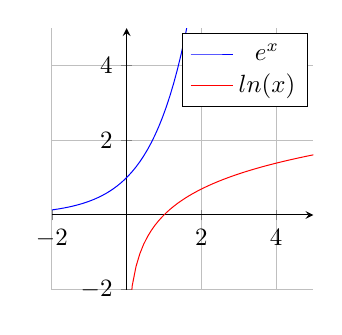
\begin{tikzpicture}[scale=0.9]
	\begin{axis}[
	width=200,
	height = 150,
	ymin=-2,
	ymax=5,
	xmin=2,
	xmax=1,
	samples=100,
	grid=both,
	no markers,
	axis equal,
	axis x line=center,
	axis y line=center,
	]

		\addplot  {e^x};
		\addlegendentry{$e^x$}
		\addplot {ln (x)};	
		\addlegendentry{$ln (x)$}
	\end{axis}
\end{tikzpicture}

\begin{definition}[Exponentialfunktion]
	$e^x := \liminfty{n} (1 + \frac{x}{n})^n = \sum_{k=0}^{\infty} \frac{x^k}{k!}$
	\begin{description} [noitemsep]
		\item Grenzwerte: $\liminfty{x} e^x = \infty$, $\limninfty{x} e^x = 0$, $\limto{x}{0} e^x = 1$
		\item Ableitung: $\frac{\partial}{\partial x}(e^x) = e^x$, $\frac{\partial}{\partial x}(e^{-x}) = -e^{-x}$		
		\item Abschätzung: $ 0 \leq 1 + x \leq e^x$,  $x < 1 \rightarrow e^x \leq \frac{1}{1 - x}$ 
		\item Rechenregeln: $e^x \cdot e^y = e^{x+y}$, $e^x \div e^y = e^{x-y}$
		\item Weitere Eigenschaften: stetig auf $\realset$, differenzierbar auf $\realset$, streng monoton wachsend, Wertemenge: $(0, \infty)$, $\liminfty{x} \frac{e^x}{x^m} = \infty$, $\limdown{x}{0} \frac{e^x - 1}{x} = 1$
		\item Komplexe Exponentialfunktion: $e^{x+iy} = e^x(cos(y) + i sin(y)) \rightarrow e^{iy} = cos(y) + i sin(y)$
		\item Matrix-Exponentialfunktion für $A \in \realset^{n \times n}$: $e^A := \sum_{i = 0}^\infty \frac{A^k}{k!}$
	\end{description}
\end{definition}

\begin{definition}[Logarithmusfunktion]
	$ln(e^x) := x$, $ln : (0, \infty) \rightarrow \realset$
	
	\begin{description} [noitemsep]
		\item Grenzwerte: $\liminfty{x} ln (x) = \infty$, $\limdown{x}{0} ln (x )= - \infty$
		\item Ableitung: $\frac{\partial}{\partial x} (ln(x)) = \frac{1}{x}$, $\frac{\partial}{\partial x} (ln(x + a)) = \frac{1}{x + a}$
		\item Abschätzung: für $x > 1$ gilt $1 - \frac{1}{x} < ln(x) < x - 1$
		\item Rechenregeln: $ln(xy) = ln(x) + ln(y)$, $ln(x \div y) = ln(x) - ln(y)$, $ln(x^k) = k \cdot ln(x)$
		\item Weitere Eigenschaften: stetig auf $(0,\infty)$, differenzierbar auf $(0,\infty)$, streng monoton wachsend, Wertemenge: $(- \infty, \infty)$, $\limdown{x}{0} x \cdot ln(x) = 0$, $\lim_{x \mapsto \infty} \frac{x}{ln(x)^n} = \infty$,  $\liminfty{x} \frac{ln(x)}{ln(ln(x))} = \infty$,  $\limdown{x}{0} \frac{ln(1+x)}{x} = 1$
	\end{description}
\end{definition}

\begin{definition}[Allgemeine Logarithmus - und Potenzfunktion]
 $\medspace$	\\ $x > 0, a \in \realset$ : $x^a = e^{ln(x^a)} = e^{a ln(x)}$ \\ $b^x = y \leftrightarrow x = log_b \leftrightarrow y = \frac{ln (y)}{ln(b)}$
	\begin{description} [noitemsep]
		\item Grenzwerte: $\liminfty{x} x^a = \begin{cases}
		+ \infty & a > 0 \\ 
		1        & a = 0  \\
		0        & a < 0
		\end{cases} \medspace \medspace $,
		$\limdown{x}{0} x^a = \begin{cases}
		0        & a > 0 \\ 
		1        & a = 0  \\
		+ \infty & a < 0
		\end{cases}$,\\
		 $\liminfty{x} \frac{x^a}{b^x} = 0$, $a > 0 \rightarrow \limdown{x}{0} x^a ln(x) = 0$, $\limdown{x}{0} \frac{ln(1+x)}{x} = 1$
		\item Ableitung: $\frac{\partial}{\partial x} (x^a) = a x^{a - 1}$, $\frac{\partial}{\partial x}(b^x) = ln(x) \cdot b^x$
		\item Rechenregeln: $x^{\frac{m}{n}} = \sqrt[m]{x^n} = (\sqrt[m]{x})^n$
	\end{description}
\end{definition}

\section{Trigonometrische Funktionen}

\begin{definition}[Einheitskreis]
Sinus und Kosinus beschreiben die Länge der Ankathete bzw. Gegenkathete im Einheitskreis.

\begin{multicols}{2}
	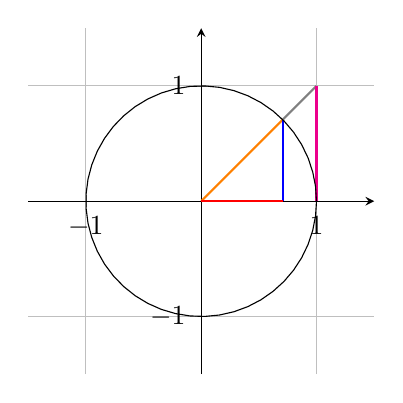
\begin{tikzpicture}
	\begin{axis}[
		width=170,
		height = 170,
		ymin=-1.5,
		ymax=1.5,
		xmin=-1.5,
		xmax=1.5,
		samples=100,
		grid=both,
		no markers,
		axis x line=center,
		axis y line=center,
	]
		\addplot [thick, orange, domain=0:0.707]{x)};
		\addplot [thick, blue] coordinates {(0.707,0)(0.707,0.707)};
		\addplot [thick, domain=0:0.707, red]{0};
		\addplot [thick, gray, domain=0.707:1]{x)};
		\addplot [thick, magenta] coordinates {(1,0)(1,1)};		
		\addplot [domain=0:2*pi,samples=50]({cos(deg(x))},{sin(deg(x))});
	\end{axis}
	\end{tikzpicture}
	\begin{itemize}[label={}, noitemsep]
		\item \textcolor{red}{Ankathete} $= cos(\phi) = a$
		\item \textcolor{blue}{Gegenkathete} $= sin(\phi) = b$
		\item \textcolor{orange}{Hypthenuse} $= 1 \overset{\text{Pythagoras}}{=} cos(\phi)^2 + sin(\phi)^2 = c$	
		\item \textcolor{magenta}{Tangente(x)} $= tan(\phi)$			
		\item $\pi := \frac{\textnormal{Kreisumfang U}}{\textnormal{Durchmesser d}} \overset{\text{Einheitskreis}}{=} \frac{U}{2} \leftrightarrow 2 \pi = U $
		\item $\rightarrow$ Kosinus und Sinus sind $2 \pi$ periodisch
		\item $\rightarrow cos(2 \pi x) = cos(x)$, $sin(2 \pi x) = sn(x)$
	\end{itemize}
\end{multicols}
\end{definition}

\begin{definition}[Rechtwinkliges Dreieck]
	Der (Ko)sinus eines Winkels beschreibt das Verhältnis der Länge der \textcolor{red}{Ankathete}/ \textcolor{blue}{Gegenkathete} zur \textcolor{orange}{Hypothenuse} eines rechtwinkligen Dreiecks
\end{definition}

\begin{multicols}{2}
\begin{tikzpicture}[scale=0.8]
\coordinate (a) at (4.4,0) {};
\coordinate (b) at (0,0) {};
\coordinate (c) at (2,2) {};
\draw[thick,red] (b) -- (c) node [midway, above, sloped] (TextNode) {a};
\draw[thick,blue] (c) -- (a) node [midway, above, sloped] (TextNode) {b};
\draw[thick,orange] (b) -- (a) node [midway, above, sloped] (TextNode) {c};
\draw pic["$\alpha$", draw=black, <->, angle eccentricity=1.2, angle radius=1cm]
{angle=a--b--c};
\draw pic["$90^{\circ}$", draw=black, <->, angle eccentricity=0.5, angle radius=1cm]
{angle=b--c--a};
\end{tikzpicture}
	\begin{itemize}[label={}, noitemsep]
	\item $cos (\alpha) = \frac{a}{c} = \frac{| \medspace \vec{a} \medspace|}{|\medspace \vec{c} \medspace |}$
	\item $sin (\alpha) = \frac{b}{c} = \frac{| \medspace \vec{b} \medspace|}{|\medspace \vec{c} \medspace |}$	
\end{itemize}
\end{multicols}

\begin{definition}[Skalarprodukt in geometrischer Definition]
	Das Skalarprodukt ordnet zwei Vektoren $a,b$ ein Skalar zu, das die Ähnlichkeit der Richtung beschreibt (, d.h. $1$ = identisch, $0$ = senkrecht).
	\begin{equation*}
	\langle a, b \rangle = |a| \cdot |b| \cdot cos(\alpha) = a^2 + b^2
	\end{equation*}
\end{definition}

\begin{definition}[Kreuzprodukt]
	Das Kreuzprodukt ordnet zwei Vektoren $a,b$ ein Vektor zu, der senkrecht auf beiden steht und als Länge den Flächeninhalt des durch $a,b$ aufgespannten Parallelogramms hat.
	
	\begin{multicols}{2}
			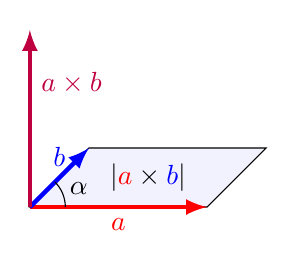
\begin{tikzpicture}[scale=0.75]
		\draw[-,fill=white!95!blue](0,0)--(3,0)--(4,1)--(1,1)--cycle;
		\node at (2,0.5) {$|\textcolor{red}{a}\times \textcolor{blue}{b}|$};
		\draw[ultra thick,-latex,red](0,0)--(3,0)node[midway,below]{$a$};
		\draw[ultra thick,-latex,blue](0,0)--(1,1)node[midway,above]{$b$};
		\draw[ultra thick,-latex,purple!50!purple](0,0)--(0,3)node[pos=0.7,right]{$a\times b$};
		\draw (0.6,0) arc [start angle=0,end angle=45,radius=0.6]
		node[pos=0.7,right]{$\alpha$};
		\end{tikzpicture}
		
		\begin{equation*}
			a \times b = det(e_3 , a , b) = \begin{pmatrix}
			 a_2b_3 - a_3b_2 \\
			 a_3b_1 - a_1b_3 \\
			 a_1b_2 - a_2b_1
			\end{pmatrix}
		\end{equation*}
	\end{multicols}
\end{definition}

\begin{definition}[Analytisch]
	Analytische Definition
	\begin{multicols}{2}
		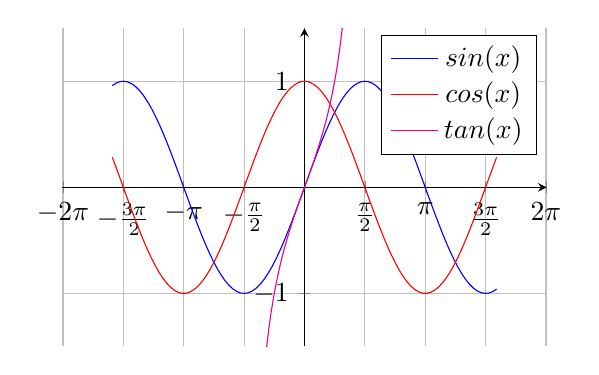
\begin{tikzpicture}
		\begin{axis}[
		width=220,
		height = 160,
		ymin=-1.5,
		ymax=1.5,
		xmin=-6.3,
		xmax=6.3,
		samples=100,
		grid=both,
		no markers,
		axis x line=center,
		axis y line=center,
		    xtick={
			-6.28318, -4.7123889, -3.14159, -1.5708,
			1.5708, 3.14159, 4.7123889, 6.28318
		},
		    xticklabels={
			$-2\pi$, $-\frac{3\pi}{2}$, $-\pi$, $-\frac{\pi}{2}$,
			$\frac{\pi}{2}$, $\pi$, $\frac{3\pi}{2}$, $2\pi$
		}
		]
		\addplot  {sin (deg(x))};
		\addlegendentry{$sin (x)$}
		\addplot {cos (deg(x))};	
		\addlegendentry{$cos (x)$}
		\addplot [magenta, domain=-1.5:1.5]{tan (deg (x)};
		\addlegendentry{$tan (x)$}
		\end{axis}
		\end{tikzpicture}
		
		\begin{itemize}[label={}, noitemsep]
			\item $sin(x)  = \sum_{k = 0}^{\infty} (-1)^k \cdot \frac{x^{2k+1}}{(2k +1)!} \overset{\text{Euler}}{=} \frac{1}{2i}(e^{ix} - e^{-ix})$ 
			\item $cos(x)  = \sum_{k = 0}^{\infty} (-1)^k \cdot \frac{x^{2k}}{(2k)!}      \overset{\text{Euler}}{=} \frac{1}{2} (e^{ix} + e^{-ix})$
			\item $\rightarrow cos(x) = sin(x + \frac{\pi}{2})$, $sin(x) = cos(x - \frac{\pi}{2})$ 	
			\item $tan : (- \frac{\pi}{2}, \frac{\pi}{2}) \rightarrow (-\infty, \infty) : x \rightarrowtail \frac{sin(x)}{cos(x)}$
	\end{itemize}
	\end{multicols}
\end{definition}

\begin{definition}[Eigenschaften]
	Für Sinus, Kosinus und Tangens gilt:
	\begin{description}[noitemsep]
		\item $sin(0) = 0, sin( \frac{\pi}{2})=1, sin(\pi) = 0, sin(\frac{3 \pi}{2}) = -1, sin(2 \pi) = 0, sin(\frac{\pi}{3}) = \frac{\sqrt{3}}{2}$. In general $sin(x) = sin(x + 2 \pi)$
		\item $cos(0) = 1, cos (\frac{\pi}{2}) = 0, cos (\pi) = 1, cos(\frac{3 \pi}{2}) = 0, cos (2 \pi) = 1, cos(\frac{\pi}{3}) = \frac{1}{2}$. In general $cos(x) = cos(x + 2 \pi)$
		\item $tan(0) = 0, tan(\pi) = 0, tan(2 \pi) = 0 \dots$ 
		\item Ableitung: $\frac{\partial}{\partial x}(cos(x)) = -sin(x), \frac{\partial}{\partial x}(sin(x)) = cos(x)$, \\ $\frac{\partial}{\partial x}(tan(x)) = \frac{1}{cos(x)^2} = 1 + tan(x)^2$
		\item Grenzwerte $\limto{x}{0} \frac{sin(x)}{x} = 1, \limto{x}{0} \frac{1 - cos(x)}{0.5x} = 1, \limdown{x}{0} \frac{tan (x)}{x} = 1$
		\item Rechenregeln: $cox(-x) = cos(x), sin(-x) = -sin(x)$ \\ $cos(x \pm y) = cos(x)cos(y) \pm sin(x)sin(y)$, \\ $sin(x \pm y) = sin(x)cos(y) \pm sin(y)cos(x)$
		\item Weitere Eigenschaften: stetig und differenzierbar auf dem gesamten Definitionsbereich
	\end{description}
\end{definition}


\begin{definition}[Umkehrfunktionen]
Für Sinus, Kosinus und Tangens seien die folgenden Umkehrfunktionen definiert:
	\begin{multicols}{2}
		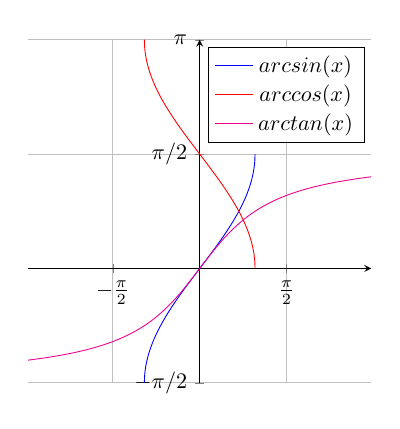
\begin{tikzpicture}[scale=0.8]
			\begin{axis}[
			width=200,
			height = 200,
			domain=-3.1:3.1, 
			samples=500, 
			axis x line=center,
			axis y line=center,
			xtick={-3.14,-1.57,0,1.57,3.14}, 
			ytick={-1.57,1.57,3.14}, 
			xticklabels={$-\pi$, $-\frac{\pi}{2}$, $0$, $\frac{\pi}{2}$, $\pi$},
			yticklabels={$-\pi$/2,$\pi$/2,$\pi$},
			grid=both]
			\addplot[color = blue,domain=-1:1]  {asin(x)/180*pi};
			\addlegendentry{$arcsin (x)$}
			\addplot[color = red, domain=-1:1]  {acos(x)/180*pi};
			\addlegendentry{$arccos (x)$}
			\addplot[color = magenta]  {atan(x)/180*pi};
			\addlegendentry{$arctan (x)$}
			\end{axis}
		\end{tikzpicture}
		\begin{description}[noitemsep]
			\item $arcsin : [-1,1] \rightarrow [0, \pi] : x \mapsto sin^{-1}(x) $
			\item $arccos : [-1,1] \rightarrow [-\frac{\pi}{2},\frac{\pi}{2}] : x \mapsto cos^{-1}(x) $
			\item $arctan : \realset \rightarrow [-\frac{\pi}{2},\frac{\pi}{2}] : x \mapsto tan^{-1} $
		\end{description}
	\end{multicols}
\end{definition}

\begin{definition}[Hyperbolische Funktionen]
	
	Der hyperbolische Sinus, Kosinus und Tangens kann definiert werden als:
\begin{multicols}{2}	
	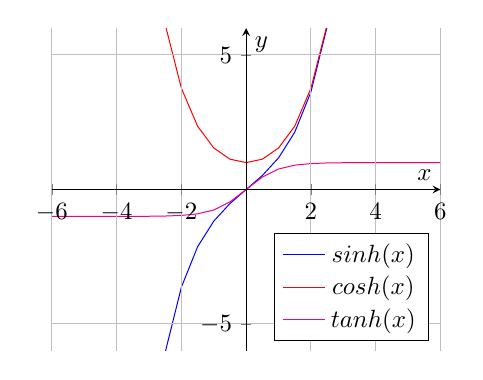
\begin{tikzpicture}[scale=0.9]
		\begin{axis}[
		xmin=-6, xmax=6,
		ymin=-6, ymax=6,
		axis lines=center,
		axis on top=true,
		domain=-6:6,
		ylabel=$y$,
		xlabel=$x$,
		scale=0.8,
		grid=both,
		legend pos=south east
		]
		\addplot [mark=none,draw=blue] {sinh(\x)};
		\addlegendentry{$sinh (x)$}
		\addplot [mark=none,draw=red] {cosh(\x)};
		\addlegendentry{$cosh (x)$}
		\addplot [mark=none,draw=magenta] {tanh(\x)};
		\addlegendentry{$tanh (x)$}
		\end{axis}
	\end{tikzpicture}
		\begin{description}[noitemsep]
		\item $sinh : \realset \rightarrow \realset : x \mapsto \frac{e^x - e^{-x}}{2} $
		\item $cosh : \realset \rightarrow [1,\infty) : x \mapsto \frac{e^x + e^{-x}}{2} $
		\item $tanh : \realset \rightarrow [-1, 1] : x \mapsto \frac{sinh(x)}{cosh(x)} = \frac{e^x- e^{-x}}{e^x + e^{-x}} $
		\end{description}
\end{multicols}
\end{definition}

\section{Komplexe Zahlen}

\begin{definition}
	Als Erweiterung der reellen Zahlen sei definiert:
	\begin{description}[noitemsep]
		\item $z \in \complexset, z = x + iy$, wobei $x,y \in \realset$ und $i := \sqrt{-1} \leftrightarrow i^2 = -1$
		\item $x := Re(z)$ nennt man \emph{Realteil} von $z$, $y := Im(z)$ heißt \emph{Imaginärteil} von $z$
		\item $\bar{z} = z^* := x - iy, |z| = \sqrt{x^2 + y^2}$
		\item $\rightarrow Re(z) = \frac{z + \bar{z}}{2}, Im(z) = \frac{z - \bar{z}}{2}$
	\end{description}
\end{definition}

\begin{definition}[Polardarstellung]
	Anstelle die Zahleneben $x,y$ einer komplexen Zahl zu verwenden, lässt sich alternativ die Länge $c$ der Zahl sowie der Winkel $\phi$ zur reellen Achse benutzen:
	
	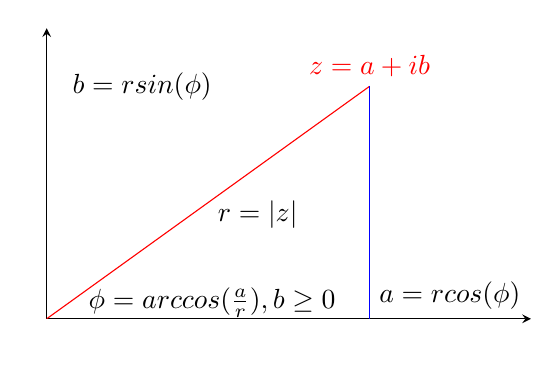
\begin{tikzpicture}
	\begin{axis}[
	ticks=none,
	domain=0:2,
	width=220,
	height=150,
	xmax=1.5,
	ymax=1.25,
	axis x line=center,
	axis y line=center,
	xtick={0, 1}, 
	ytick={1, 0},
	xlabel style={at={(axis description cs:0.5,-0.0)},anchor=north},
	xlabel={$\realset$},
	ylabel style={at={(axis description cs:-0.0,.5)},rotate=90,anchor=south},
	ylabel={$\complexset$}]
	
	\addplot [red, domain=0:1]{x}  node[above,pos=1] {$z = a + ib$};
	\addplot [blue, domain=0:1] coordinates {(1,0)(1,1)};	
	\node[right] at (1, 0.1)  {$a = r cos(\phi)$} ;
	\node[right] at (0.5, 0.45)  {$r = |z|$} ;
	\node[right] at (0.05, 1)  {$b = r  sin(\phi)$} ;
	\node[right] at (0.1, 0.07)  {$\phi = arccos(\frac{a}{r}), b \geq 0$} ;
	\end{axis}
	\end{tikzpicture}
	
	$(r, \phi) $ bezeichnet man als Polarkoordinaten der komplexen Zahl. Der Wert des Winkels $\phi$ wird auch als \emph{Argument} bezeichnet. Algebraisch ist es der Wert sodass $z = r (cos \phi + i sin \phi) = re^{i\phi}$
	
\end{definition}

\begin{satz}[Euler'sche Formel]
	$e^{iy} = cos(x) + i sin(x)$
	
	\begin{description}[noitemsep]
		\item $\rightarrow e^{it}$ durchläuft den Einheitskreis 
		\item $\rightarrow e^{i \cdot 0} = e^{i \cdot 2k\pi} = 1, e^{-i\pi} = -1$
	\end{description}
	
\end{satz}

\pagebreak

\section{Frequenzanalyse und Fourier-Reihe}
\begin{definition}[Trigonometrisches Polynom]
	Man definiert analog zu regulären Polynomen Polynome mit trigonometrischen Funktionen mit Grad $n$ als Basis im Intervall $[-\frac{T}{2}, \frac{T}{2}]$ 
	\begin{align*}
		F_n(t) := \frac{a_0}{2} + \sum_{k=1}^{n} (a_k cos(k\omega t) + b_k sin(k \omega t))
	\end{align*}
	wobei $\omega := \frac{2 \pi}{T}$ und $a_k, b_k$ Fourierkoeffizienten genannt werden.
\end{definition}

\begin{satz}
	Unter Rücksichtnahme der Norm für Funktionen, $||f|| := \int_a^b |f(x)|^2$, minimieren für eine stetige, beschränkte Funktion $f$ die folgenden Koeffizienten das approximierende trigonometrische Polynom;
	
	\begin{align*}
		a_k = \frac{2}{T} \int_{-\frac{T}{2}}^{\frac{T}{2}} cos(k \omega t)f(t) dt,
		b_k = \frac{2}{T} \int_{-\frac{T}{2}}^{\frac{T}{2}} sin(k \omega t)f(t) dt,	
	\end{align*}
	
	An jeder Stelle, an der $f$ differenzierbar ist, konvergiert dann $F_n$ für $n \rightarrow \infty$ gegen den Funktionswert. Wir schreiben
	
	\begin{align*}
		f(t) = \frac{a_0}{2} + \sum_{k=1}^{\infty}a_k cos(k \omega t) + b_k sin(k \omega t)
	\end{align*}
\end{satz}

\begin{definition}[Spektrum]
	Für eine Funktion dargestellt als Fourierreihe, z.B. $f(t) = cos()$
\end{definition}

\pagebreak

\section{Differenzierbarkeit}

\begin{definition}[Landau-Symbole]
	Seien $f,g : \realset \rightarrow \complexset$ Funktionen, $x_0 \in \realset$
	\begin{description}[noitemsep]
		\item $f(x) = \mathcal{O}(g(x))$ für $x \rightarrow x_0$ falls: $\exists \epsilon > 0: \exists c > 0 : \forallxinreal$ mit $|x - x _0| < \epsilon : |f(x)| < c \cdot |g(x)|$, d.h. in einer Umgebung von $x_0$ wird $f(x)$ von $g(x)$ mal einer Konstante beschränkt.
		\item $f(x) = o(g(x))$ für $x \rightarrow x_0$ falls $\lim_{x \rightarrow x_0} \frac{f(x)}{g(x)} = 0 $
		\item $f(x) = \mathcal{O}(g(x))$ für $x \rightarrow \infty$ falls: $\exists M > 0: \exists c > 0 : \forall x > M : |f(x)| < c \cdot |g(x)|$, d.h. ab einer Schranke $M$ wird $f(x)$ durch $g(x)$ beschränkt.
		\item $f(x) = \mathcal{O}(g(x))$ für $x \rightarrow -\infty$ falls: $\exists M > 0: \exists c > 0 : \forall x < -M : |f(x)| < c \cdot |g(x)|$, d.h. ab einer Schranke $M$ wird $f(x)$ durch $g(x)$ beschränkt.	
		\item $f(x) = o(g(x))$ für $x \rightarrow x_0 \in \{\pm \infty\}$ falls $\lim_{x \rightarrow x_0} \frac{f(x)}{g(x)} = 0 $
	\end{description}
\end{definition}

\begin{definition}[Differenzierbarkeit]
	Eine Funktion $\f{I}{\realset}, I \subseteq \realset$ heißt differenzierbar in $x_0 \in I$, falls $\lim_{x \rightarrow x_0} \frac{f(x) - f(x_0)}{x - x_0}$ bzw. $\lim_{h \rightarrow 0} \frac{f(x_0 + h) - f(x_0)}{h}$ existiert. Man schreibt dafür $f'(x_0)$ (Lagrange), $\frac{\partial f}{\partial x_0}$ (Leibniz). Ist $f$ differenzierbar für alle $x_0 \in I$, so heißt $f$ differenzierbar.
\end{definition}

\begin{satz}[Rechenregeln differenzierbrer Funktionen]
	Seien $f,g : I \subseteq \realset \rightarrow \realset$ in $x \in I$ differenzierbar, $c \in \realset$.
	\begin{description}[noitemsep]
		\item $(c \cdot f)'(x) = c \cdot f'(x) $
		\item $(f + g)'(x) = f'(x) + g'(x) $
		\item $(f \cdot g)'(x) = f'(x) g(x) + f(x)g'(x) $  (Produktregel)
		\item $(\frac{f}{g})'(x) = \frac{f'(x) g(x) - f(x)g'(x)}{g(x)^2} $	 (Quotientenregel)
	\end{description}
\end{satz}

\begin{satz}[Kettenregel]
	Sei $\f{ D \subseteq \realset}{\realset}$, $g : E \subseteq \realset \rightarrow \realset$ und $g(E) \subseteq D$. Sei $x_0$ innererer Punkt von $E$, $g(x_0)$ innerer Punkt von $D$. Sei $g$ in $x_0$ und $f$ in $g(x_0)$ differenzierbar. Dann gilt: $(f \circ g)'(x_0) = f'(g(x_0)) \cdot g'(x_0)$
 \end{satz}

\begin{satz}[Ableitung der Umkehrfunktion]
	Sei $\f{I \subseteq \realset}{J \subseteq \realset} $ bijektiv und differenzierbar in $y_0$. Dann ist $f^{-1} : J \rightarrow I$ differenzierbar in $y_0$ und $(f^{-1})'=\frac{1}{f'(f^{-1}(y_0))}$
\end{satz}



\begin{satz}[Elementare Ableitungen]
	Es gelten folgende Ableitungen:
	\begin{multicols}{2}
		\begin{description}[noitemsep]
			\item $(c)' = 0$
			\item $(x^a)'=ax^{a-1}$
			\item $(e^x)'=e^x$
			\item $sin'(x) = cos(x)$
			\item $cos'(x) = -sin(x)$
			\item $tan'(x) = \frac{1}{cos(x)^2} = 1 + tan(x)^2$
			\item $ln'(x) = \frac{1}{x}$
			\item $arcsin'(x) = \frac{1}{\sqrt{1 -x^2}}$	
			\item $arccos'(x) = - \frac{1}{\sqrt{1 - x^2}}$	
			\item $arctan'(x) = \frac{1}{1 + x^2}$
			\item $(a^x)' = a^x ln(a)$
			\item $ln(u(x))'=\frac{u'(x)}{u(x)}$
		\end{description}
	\end{multicols}
\end{satz}

\section{Anwendungen der Ableitung}

\begin{satz}
	Sei $\fab$ differenzierbar auf $(a,b)$. Wenn $f$ in $x_0$ ein lokales Extremum besitzt, dann gilt $f'(x_0) = 0$.
\end{satz}

\begin{satz}[Mittelwertsatz]
	Sei $\fab$ differenzierbar auf $[a,b]$, differenzierbar auf $(a,b)$. Dann gibt es ein $\xi \in (a,b)$ sodass $\frac{f(b) - f(a)}{b - a} = f'(\xi)$.
\end{satz}

\begin{satz}[Satz von Rolle]
	Gilt neben dem Mittelwertsatz zusätzlich $f(a) = f(b)$, dann gibt es ein $\xi \in (a,b)$ sodass $f'(\xi) = 0$.
\end{satz}

\begin{satz}[Monotonie und Ableitungen]
	\begin{description}[noitemsep]
		\item $\forallin{x}{(a,b)}: f'(x) > 0 \rightarrow f$ ist auf $[a,b]$ streng monoton wachsend
		\item $\forallin{x}{(a,b)}: f'(x) < 0 \rightarrow f$ ist auf $[a,b]$ streng monoton fallend
		\item $\forallin{x}{(a,b)}: f'(x) \geq 0 \rightarrow f$ ist auf $[a,b]$ monoton wachsend
		\item $\forallin{x}{(a,b)}: f'(x) \leq 0 \rightarrow f$ ist auf $[a,b]$ monoton fallend
	\end{description}
\end{satz}

\begin{satz}
	Sei $\fabex$ differenzierbar, sei $f'(x_0) = 0, x_0 \in (a,b)$.
	\begin{description}[noitemsep]
		\item $f' \geq 0$ in $(a, x_0)$ und $f' \leq 0$ in $(x_0, b) \rightarrow x_0$ ist globales Maximum
		\item $f' \leq 0$ in $(a, x_0)$ und $f' \geq 0$ in $(x_0, b) \rightarrow x_0$ ist globales Minimum
	\end{description}
\end{satz}

\begin{satz}
	Seien $f,g : (a,b) \rightarrow \realset$ differenzierbar und $f' = g'$ auf $(a,b)$. Dann gibt unterscheiden sich $f,g$ nur um eine Konstante, d.h. $\exists c \in \realset : f = g + c$ auf $(a,b)$.
\end{satz}

\begin{satz}[L'Hospital]
	Seien $a,b \in \realset \cup \{+ \infty, - \infty\}$. Seien $f, g : (a,b) \rightarrow \realset$ differenzierbar mit $g'(x) \neq 0$. Sei $x_0 \in (a,b)$ und es gelte:
	\begin{enumerate}[noitemsep]
		\item $\lim_{x \rightarrow x_0} f(x) = 0 = \lim_{x \rightarrow x_0} g(x)$ oder
		\item$\lim_{x \rightarrow x_0} f(x) = \pm \infty = \lim_{x \rightarrow x_0} g(x)$
	\end{enumerate}
	Falls $\lim_{x \rightarrow x_0} \frac{f'(x)}{g'(x)}$ existiert, gilt: $\lim_{x \rightarrow x_0} \frac{f(x)}{g(x)} = \lim_{x \rightarrow x_0} \frac{f'(x)}{g'(x)}$.
\end{satz}

\begin{definition}
	Für zweimal differenzierbares $\fabex$ gilt:
	\begin{enumerate}[noitemsep]
		\item $f$ heißt \emph{konvex} $\leftrightarrow f'' \geq 0$ auf $(a,b)$
		\item $f$ heißt \emph{konkav} $\leftrightarrow f'' \leq 0$ auf $(a,b)$		
	\end{enumerate}
\end{definition}

\begin{satz}
	Sei $\fabex$ zweimal differenzierbar und $f'(x_0)=0$ und $\exists x_0 \in (a,b) : f'(x_0) = 0$.
	
	\begin{enumerate}[noitemsep]
		\item $f''(x_0) > 0 \rightarrow f$ besitzt in $x_0$ ein striktes lokales Minimum
		\item $f''(x_0) < 0 \rightarrow f$ besitzt in $x_0$ ein striktes lokales Maximum	
	\end{enumerate}
\end{satz}

\begin{satz}[Differenzierbarkeit und Stetigkeit]
	Ist $f$ differenzierbar, so ist $f$ stetig.
\end{satz}

\pagebreak

\section{Integrale}

\begin{multicols}{2}
	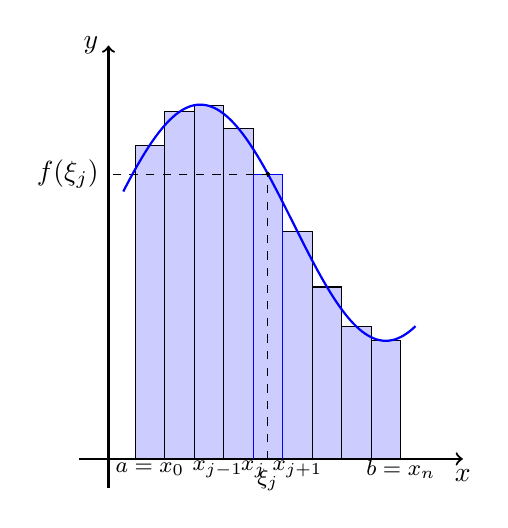
\begin{tikzpicture}[scale=0.75]
	\def\a{0.7}
	\def\b{4.2}
	\def\c{2.7}
	\def\L{0.5} % width of interval
	
	\pgfmathsetmacro{\Va}{2*sin(\a r+1)+4} \pgfmathresult
	\pgfmathsetmacro{\Vb}{2*sin(\b r+1)+4} \pgfmathresult
	\pgfmathsetmacro{\Vc}{2*sin(\c r+1)+4} \pgfmathresult
	
	\draw[->,thick] (-0.5,0) -- (6,0) coordinate (x axis) node[below] {$x$};
	\draw[->,thick] (0,-0.5) -- (0,7) coordinate (y axis) node[left] {$y$};
	\foreach \f in {0.7,1.2,1.7,2.2,...,4.7} {\pgfmathparse{2*sin(\f r+1)+4} \pgfmathresult
		\draw[fill=blue!20] (\f-\L/2,\pgfmathresult |- x axis) -- (\f-\L/2,\pgfmathresult) -- (\f+\L/2,\pgfmathresult) -- (\f+\L/2,\pgfmathresult |- x axis) -- cycle;}
	\node at (\a-\L/2+0.25,-5pt) {\footnotesize{$a=x_0$}};
	\node at (\b+\L/2+\L,-5pt) {\footnotesize{$b=x_n$}};
	\draw[blue] (\c-\L/2,0) -- (\c-\L/2,\Vc) -- (\c+\L/2,\Vc) -- (\c+\L/2,0);
	\draw[dashed] (\c,0) node[below] {\footnotesize{$\xi_j$}} -- (\c,\Vc) -- (0,\Vc) node[left] {$f(\xi_j)$};
	\node at (\a+5*\L/2 - 0.1,-5pt) {\footnotesize{$x_{j-1}$}};
	\node at (\a+7*\L/2,-5pt) {\footnotesize{$x_j$}};
	\node at (\a+5*\L,-5pt) {\footnotesize{$x_{j+1}$}};
	\draw[blue,thick,smooth,samples=100,domain=0.25:5.2] plot(\x,{2*sin(\x r+1)+4});
	\filldraw[black] (\c,\Vc) circle (.03cm);
	\end{tikzpicture}
	
	\begin{definition}[Riemann-Summe]
		Sei $Z$ eine Zerlegung von $[a,b]$ : $a = x_0 < x_1 < \dots < x_{n-1} < x_n = b$. Die Feinheit von $Z$ ist $|Z| = max_{1 \leq j \leq n}\{|x_j - x_{j-1}|\}$. Gegeben sei ein Zerlegung $Z$. Sei $\xi \in [x_{j-1}, x_j]$ mit $1 \leq j \leq n$ beliebig. $S_Z = \sum_{j=1}^{n} f(\xi) \cdot (x_j-x_{j-1})$ heißt \emph{Riemann-Summe}, wobei $f(\xi)$ Höhe der Rechtecksflächen.
	\end{definition}
\end{multicols}

\begin{definition}[Riemann-integrierbar]
	$\fab$ heißt \emph{Riemann-integrierbar}, falls für alle Zerlegungsfolgen $(Z_n)_{n \in \naturalset}$ mit Feinheit $|Z_n| \overset{n \rightarrow \infty}{\rightarrow} 0$ die zugehörigen Riemann-Summen $S_{Z_n}$ für jede Wahl der Zwischenpunkte gegen den selben Grenzwert $I(f)$ konvergieren: $\liminfty{n} \sum_{j=1}^n f(\xi_f) \cdot (x_j - x_{j-1}) = I(f) := \int_{a}^{b}f(x) dx$
\end{definition}

\begin{satz}[Rechenregeln für Integrale]
	Seien $f,g : [a,b] \rightarrow \realset$ Riemann-integrierbar, $\delta, \mu \in \realset$. Es gilt:
	\begin{description}[noitemsep]
		\item $\int_{a}^{a} f(x) dx = 0$, $\int_{b}^{a} f(x) dx = - \int_{a}^{b} f(x) dx$, $\int_{a}^{b} 1 dx = \int_{a}^{b} dx = b - a$
		\item $\int_{a}^{b} f(x) dx \geq 0$ für $f \geq 0$ auf $[a,b]$, $\int_{a}^{b} \delta f(x) + \mu g(x) dx = \delta \int_{a}^{b}f(x) dx + \mu \int_{a}^{b} g(x) dx$
		\item $\int_{a}^{b} f(x) dx = \int_{a}^{c} f(x) dx + \int_{c}^{b} f(x) dx$ für $a < b < c$
	\end{description} 
\end{satz}

\begin{satz}
	Jede stetige Funktion ist Riemann-integrierbar.
\end{satz}

\begin{satz}[Mittelwertsatz der Integralrechnung]
	Sei $\fab$ stetig, $\gab$ integrierbar und $g \geq 0$ oder $g \leq 0$. Dann gibt es ein $\xi \in [a,b]$ sodass $\int_{a}^{b}f(x)g(x) dx = f(\xi) \cdot \int_{a}^{b} g(x) dx$. Für $g=1$ ergibt sich der Spezialfall $\int_{a}^{b}f(x)dx = f(\xi) \cdot \int_{a}^{b} dx = f(\xi) \cdot (b - a)$
\end{satz}

\begin{satz}[Hauptsatz der Differential und Integralrechnung]
	Sei $\fab$ stetig. Die Funktion $\functionab{F}$ mit $F(x) = \int_{a}^{x} f(t) dt$ ist in jedem $x \in (a,b)$ differenzierbar und es gilt: $F'(x) = f(x)$.
\end{satz}

\begin{satz}
	Sei $\fab$ stetig und $\functionab{F}$ Stammfunktion von $f$. Dann gilt: $\int_{a}^{b}f(x)dx = F(b) - F(a) := [F(x)]_a^b$. Für eine Stammfunktion von $f$ schreibt man auch $\int f(x) dx$ (unbestimmtes Integral).
\end{satz}

\begin{satz}[Partielle Integration]
	Seien $\functionab{g,f}$ stetig differenzierbar. Dann gilt:
	\begin{description}[noitemsep]
		\item $\int_{a}^{b} f(x)g'(x)dx = [f(x)g(x)]_a^b - \int_{a}^{b} f'(x)g(x)dx$
		\item $\int f(x)g'(x)dx = f(x)g(x) - \int f'(x)g(x)dx$	
	\end{description}
\end{satz}

\begin{satz}[Integration durch Substitution]
	Seien $\functionab{g,f}$ stetig differenzierbar. Dann gilt für jede stetige Funktion $\function{f}{g([a,b])}{\realset}$:
	\begin{description}[noitemsep]
		\item $\int_{a}^{b} f(g(t))g'(t) = \int_{g(a)}^{g(b)}f(x)dx$
		\item $\int f(g(t))g'(t) = \int f(x)dx$
	\end{description}
\end{satz}


\section{Potenzreihen}

\begin{definition}
	Funktionsdarstellungen der Form $f(x) = \serieskzeroinfty{a}x^k, |x| < r$ nennt man Entwicklung von $f$ in eine Potenzreihe. Die größtmögliche Gültigkeitsschranke für Konvergenz nennt man Konvergenzradius der Potenzreihe.
\end{definition}

\begin{satz}[Taylor'sche Formel]	
	Sei $f $ n+1-mal stetig differenzierbar. Wir definieren die folgenden Taylorentwicklungen um den Punkt $a \in \realset$:
	
	\begin{itemize}[noitemsep]
		\item $f(x) =  \sum_{k = 0}^n \frac{f^{(k)}(a)}{k!} \cdot (x - a)^k + R_{n+1}$
		\item $f(x + a) = \sum_{k = 0}^n \frac{f^{(k)}(x)}{k!} \cdot a^k + R_{n+1}$
		\item $f(x - a) = \sum_{k = 0}^n \frac{f^{(k)}(x)}{k!} \cdot (-a)^k + R_{n+1}$
	\end{itemize}

	$R_n$ bezeichnet dabei den Fehler bzw. das Restglied in de Entwicklung. Es kann angegeben werden mit:
	
	\begin{itemize}[noitemsep]
		\item $R_{n+1} := \frac{(x - a)^{(n + 1)}}{(n + 1)!} \cdot f^{(n + 1)}(\xi)$ (Lagrange Restglied)
		\item $R_{n+1} := \frac{1}{n!} \int_{a}^{x} (x - t)^nf^{(n+1)}(t)dt$ (Cauchy Restglied)
	\end{itemize}

	Gleichzeitig gilt: $R_{n+1} \in \BigO{a^{n+1}}$

\end{satz}


\begin{satz}
	Zu jeder Potenzreihe $\serieskzeroinfty{a}x^k$ gibt es einen Konvergenzradius sodass $\forallin{z}{\complexset}$ gilt:
	\begin{description}[noitemsep]
		\item $|z| < r \rightarrow $ die Potenzreihe konvergiert absolut
		\item $|z| > r \rightarrow $ die Potenzreihe divergiert
		\item der Fall $|z| = r$ muss gesondert betrachtet werden
	\end{description}
	Falls die Folge $\sequence{\sqrt[k]{|a|}}{k}$ konvergiert, so ist $r = \frac{1}{\liminfty{k}\sqrt[k]{|a|_k}}$
\end{satz}

\begin{definition}
	Eine Funktion heißt \emph{analytisch}, wenn sie sich mit positivem Konvergenzradius in eine Potenzreihe entwickeln lässt.
\end{definition}

\begin{satz}
	Sind $f,g$ in $x=0$ analytisch, $f(x) = \serieskzeroinfty{a}x^k, |x| < r_f$, $g(x) = \serieskzeroinfty{b}x^k, |x| < r_g$. Dann gilt:
	\begin{enumerate}[noitemsep]
		\item $f'$ ist in $x=0$ analytisch und $f'(x) = \frac{\partial}{\partial x} \serieskzeroinfty{a}x^k = \sum_{k=0}^{\infty} \frac{\partial}{\partial x}a_kx^k, |x| < r_f$
		\item Die Koeffizienten sind eindeutig $a_k = \frac{f^{(k)}(0)}{k!}, k \in \naturalset_0$
		\item Stammfunktionen sind in $x=0$ analytisch: $\int_{0}^{x}f(t)dt = \int_{0}^{x}\serieskzeroinfty{a}t^k dt= \sum_{k=0}^{\infty}\int_{0}^{x}a_k t^k dt$
		\item $f + g, f \cdot g$ sind analytisch mit
		\begin{description}
			\item $(f + g)(x) = \sum_{k=0}^{\infty} (a_k+b_k)x^k, |x|=\min\{r_f, r_g\}$
			\item $(f \cdot g)(x) = \sum_{k=0}^{\infty} \sum_{j=0}^{k} a_jb_{k-j}x^k, |x|=\min\{r_f, r_g\}$
		\end{description}
	\end{enumerate}
\end{satz}

\pagebreak

\section{Mehr über Integrale}
\begin{definition}
	Ist $f : [a,b)$ auf $[\alpha, \beta]$ integrierbar für alle $a < \beta < b$, dann heißt $\int_{a}^{b} f(x) dx = \limto{\beta}{b} \int_{a}^{\beta} f(x) dx$ \emph{uneigentliches Integral}. Analog verfährt man mit der unteren Grenze.
\end{definition}

\begin{definition}
	Ist $f : (a,b)$ auf $[\alpha, \beta]$ integrierbar für alle $a < \alpha < \beta < b$, dann heißt $\int_{a}^{b} f(x) dx = \limto{\alpha}{a} \int_{\alpha}^{c} f(x) dx + \limto{\beta}{b} \int_{c}^{\beta} f(x) dx$ \emph{uneigentliches Integral}, falls die Grenzwerte für ein $c \in (a,b)$ existieren.
\end{definition}

\begin{definition}
	Wir betrachten $f(x,y)$. Für ein festes/konstantes $x$ schreiben wir die Ableitung $y \mapsto f(x,y) : \partial y f(x,y)$ oder $\partial_2 f(x,y)$.
\end{definition}

\begin{satz}
	Sei $f : [a,b] \times [c,d]$ stetig. Es gilt:
	\begin{enumerate}[noitemsep]
		\item $F : y \mapsto \int_{a}^{b} f(x,y) dx$ ist stetig
		\item (Fubini) $\int_{c}^{d} F(y) dx= \int_{c}^{d} \int_{a}^{b} f(x,y) dx dy =  \int_{a}^{b} \int_{c}^{d} f(x,y) dy dx $
		\item Besitzt $f$ eine stetig partielle Ableitung $\partial_y$, dann ist $F$ differenzierbar mit $F'(y) = \int_{a}^{b} \partial_y f(x,y) dx$ und $\frac{\partial}{\partial y} \int_{a}^{b} f(x,y) dx = \int_{a}^{b} \frac{\partial}{\partial y} f(x,y) dx$ 
	\end{enumerate}
\end{satz}

\begin{satz}
	Sei die Funktionsfolge $f_k : [a,b] \mapsto \realset$ integrierbar und es gebe $a_k \geq 0$ sodass $|f_k| \leq a_k$ für alle $x \in [a,b]$ und $\serieskinfty{1}{a} < \infty$. \\
	$\rightarrow f(x) = \sum_{k=1}^{\infty} f_k(x)$ konvergiert und es gilt: $\int_{a}^{b}f(x)dx = \int_{a}^{b} \sum_{k=1}^{\infty} f_k(x)dx =  \sum_{k=1}^{\infty} \int_{a}^{b}f_k(x) dx$
\end{satz}

\begin{satz}
	Seien $a,b \in \mathbb{Z}$, sei $\fab$ stetig und monoton, $a < b, f \geq 0$. Es gilt
	\begin{description}[noitemsep]
		\item $f$ monoton wachsend $\rightarrow \sum_{k=a}^{b-1} f(k) \leq \int_{a}^{b}f(x)dx \leq \sum_{k=a+1}^{b}f(k)$
		\item $f$ monoton fallend  $\rightarrow \sum_{k=a+1}^{b} f(k) \leq \int_{a}^{b}f(x)dx \leq \sum_{k=a}^{b-1}f(k)$
	\end{description}
\end{satz}

\begin{satz}[Integralkriterium für Reihen]
	$\rightarrow$ siehe Blatt Reihen
\end{satz}

\begin{satz}[Riemannsche Zetafunktion]
	$\rightarrow$ siehe Blatt Reihen
\end{satz}

\begin{satz}
	Die folgenden uneigentlichen Integrale gelten: \\
	$\int_{0}^{1} \frac{1}{x^\alpha} dx = 
		\begin{cases}
			+ \infty              &, \alpha > 1 \\ 
	 		\frac{1}{1 - \alpha}  &, \alpha < 1
		\end{cases}$, 
	$\int_{1}^{\infty} \frac{1}{x^\alpha} dx = 
		\begin{cases}
			\frac{1}{\alpha - 1}  &, \alpha > 1 \\
			+ \infty              &, \alpha < 1 
		\end{cases}$
\end{satz}

\pagebreak

\section{Verallgemeinerungen für mehrere Veränderliche}

\begin{definition}[Punktmenge]
	Teilmengen der reellen Zahlen $X \subseteq \realset^n$ werden Punktmengen genannt. Elemente von $x \in X$ heißen auch Punkte

	Für eine reele Zahl $\epsilon \in \realset$ und einen Punkt $x \in \realset^n$ heißt die Menge $U(x)_\epsilon := \{ y \in \realset^n | \norm{x - y} \leq \epsilon \}$ $\epsilon$ - Umgebung von $x$ bzgl. der Norm.
\end{definition}

\begin{definition}[Beschränktheit]
	Eine Menge $M \subseteq \realset^n$ heißt beschränkt, falls es eine $\epsilon$ - Umgebung um $0$ gibt, die $M$ enthält: $M \subseteq U_\epsilon(0)$. Dies ist äquivalent dazu, dass der Abstand zweier beliebiger Punkte in $M$ beschränkt ist: $\forallin{x,y}{M} : \norm{x - y} < \epsilon$
\end{definition}

\begin{definition}[Punktfolge]
	Eine Abbildung $\function{\phi}{\naturalset}{\realset^n}$ heißt auch Punktfolge. Man schreibt für die Glieder der Punktfolge hochgestellte Indices: $x^{(k)} = (x_1^{(k)}, ..., x_n^{(k)})$, für die Folge selbst schreibt man $(x^{(k)})$. Eine Punktfolge heißt beschränkt, wenn ihre Wertemenge $\{ x^{(k)} \medspace |\medspace k \in \naturalset \}$ beschränkt ist.
\end{definition}


\begin{definition}[Grenzwerte]
	$a \in \realset^n$ heißt Grenzwert der Folge $(x^{(k)})$, falls \\ $\lim_{k \rightarrow \infty} \norm{x^{(k)} - a} = 0$. Die Folge heißt dann auch konvergent. Besitzt eine Punktfolge keinen endlichen Grenzwert, so heißt sie divergent.
	Bei konvergenten Folgen liegen in jeder $\epsilon$ Umgebung von $g$ fast alle Folgenglieder und nur endlich viele außerhalb. Eine Punktfolge konvergiert nur dann, wenn sie kompontenweise konvergiert.
\end{definition}

\begin{definition}[Funktion mehrerer Veränderlicher]
	Bei Funktionen mehrerer Veränderlicher ist der Definitionsbereich $D$ eine Teilmenge des $\realset^n$. Sie ordnet 
	jedem Punkt $x \in D \subseteq \realset^n$ eine relle Zahl zu: $\f{D \subseteq \realset^n}{\realset}$. Man nennt solche Funktionen auch skalares Feld (jeden Punkt in einem Raum wird ein skalar zugeordnet). 
	
	Ein skalares Feld $f$ heißt auf $E \subseteq D$ nach oben (unten) beschränkt, falls $f(E) = \{f(x) \medspace | \medspace x \in E\} \subseteq \realset$  nach oben (unten) beschränkt ist.´ 
\end{definition}

\begin{definition}[Grenzwerte skalarer Feldern]
	Eine Funktion $\f{D \subseteq \realset^n}{\realset}$ sei in der Umgebung von $x_0 = (x_1, ..., x_n) \in D$ definiert (aber nicht zwansweise an $x^0$ selbst). $f$ hat an der Stelle  $x_0$ den Grenzwert $a$, $a = \lim_{x \rightarrow x_0} f(x)$, genau dann wenn, für jede Folge $(x^{(k)})_{k \in \naturalset}$ aus $D$ mit $x_0 \neq x^{(k)}$ und $\lim_{k \rightarrow \infty} x^{(k)} = x_0$ gilt: $\lim_{k \rightarrow \infty} f(x^{(k)}) = a$
\end{definition}

\begin{definition}[Stetigkeit]
		Eine Funktion $\f{D \subseteq \realset^n}{\realset}$  heißt stetig im Punkt $x_0 = (x_1, ..., x_n) \in D$ wenn der Grenzwert $\lim_{x \rightarrow x_0} f(x)$ existiert und $\lim_{x \rightarrow x_0} f(x) = f(x_0)$ . $f$ heißt stetig auf der Menge $M \subseteq D$, falls $f$ in jedem Punkt $x_0 \in M$ stetig ist.
\end{definition}

\pagebreak

\section{Differentialrechnung mehrerer Veränderlicher}

\begin{definition}[partielle Ableitung]
	Sei $D \subseteq \realset^n$ offen, $\f{D}{\realset}, \xi \in D$. $F$ ist in $\xi$ nach  $x_i$ partiell differenzierbar, falls der Grenzwert
	
	\begin{align*}
		\partialf{f}{x_i} := \lim_{h \rightarrow 0} \frac{f(\xi + h \cdot e_i) - f(\xi)}{h} 
	\end{align*}
	existiert. $e_i$ bezeichnet den $i$-ten Einheitsvektor.  Wir schreiben $\frac{\partial f}{\partial x_i}$ bzw. $\partial_{x_i} f(x)$ oder $f_{x_i}(x)$ und $\partialf{f}{x_i}(\xi)$ heißt partielle Ableitung von $f$ nach $x_i$ im Punkt $\xi$.
	
	Ist $f$ in allen Punkten $\xi \in D$ partiell differenzierbaer nach $x_i$, so heißt $f$ auf $D$ partiell differenzierbar nach $x_i$. Gilt dies für alle $x_i, i=1,...,n$, so heißt $f$ partiell differenzierbar auf $D$. Sind die partiellen Ableitungen stetig, so heißt $f$ stetig partiell differenzierbar.
\end{definition}

\begin{satz}[Differentiationsregeln]
	Seien $\function{f,g}{D}{\realset}, D \subseteq \realset^n$ partiell differenzierbar. Dann gilt:
	\begin{enumerate}[noitemsep]
		\item  Linearität: $\partialf{}{x_i}(\alpha f(x) + \beta g(x)) = \alpha \partialf{f}{x_i}(x) + \beta \partialf{g}{x_i}(x) $
		\item  Produktregel: $\partialf{}{x_i}( f(x) g(x)) = \partialf{f}{x_i}(x)g(x) + f(x)\partialf{g}{x_i}(x)$
		\item  Quotientenregel: $\partialf{}{x_i}( \frac{f(x)}{g(x)}) = \frac{\partialf{f}{x_i}(x)g(x) - f(x)\partialf{g}{x_i}(x)}{g(x)^2}$ falls $g(x) \neq 0$
	\end{enumerate}
	
\end{satz}


\begin{definition}[Gradient]
	Betrachte $\function{f}{D \subseteq\realset^n}{\realset}$, deren sämtliche partiellen Ableitungen in $\xi$ nach allen $x_i$ existieren. 
	Dann nennt man den Vektor $\nabla f(x) = grad(f(x)) = \left(\begin{smallmatrix}
		\partialf{f}{x_1}(\xi) \\
		 \vdots \\
		 \partialf{f}{x_n}(\xi)
	\end{smallmatrix}\right)$ Gradient.
	Mit ihm lassen sich die Differentiationsregeln schreiben als
	\begin{itemize}[noitemsep]
		\item  $\nabla(\alpha f + \beta g) = \alpha \nabla f + \beta \nabla g$
		\item  $\nabla (fg) = \nabla (f) g + f \nabla(g)$
		\item  $\nabla (\frac{f}{g}) = \frac{1}{g^2} (\nabla (f) g - f \nabla(g))$	
	\end{itemize}
und er definiert die Richtung des steilsten Anstiegs von $f$ im Punkt $\xi$ bzgl. $\normempty_2$
\end{definition}

\begin{definition}[Partielle Ableitungen höherer Ordnung]
	Sei $D \subseteq \realset^n$ offen, $\f{D}{\realset}$. Ist $f$ auf $D$ partiell differenzierbar und sind die partiellen Ableitungen selbst wieder partiell differenzierbar, erhält man die partielle Ableitung zweiter Ordnung: 
	\begin{align*}
		\partialf{^2}{x_j x_i} := \partialf{}{x_j}(\partialf{f}{x_i})
	\end{align*}
	Analog definiert man partielle Ableitungen $k$-ter Ordnung.  Sind die partiellen Ableitungen stetig, so heißt $f$ $k-fach$ stetig (partiell) differenzierbar
\end{definition}

\begin{satz}[Satz von Schwarz]
	Sei $D \subseteq \realset^n$ offen, $\f{D}{\realset}$, $f \in \cnspace{2}{D}{\realset}$.  Dann gilt: $\partialf{^2f}{x_j \partial x_i} = \partialf{^2f}{x_i \partial x_j}$. Ist $f$ $k$-mal stetig differenzierbar, so kann man die Reihenfolge der partiellen Ableitungen bis zur Ordnung $k$ beliebig tauschen.
\end{satz}

\begin{definition}[Hesse-Matrix]
	Die Matrix $Hf(\xi) := (\partial_j \partial_i f(\xi))_{1 \leq i \leq j \leq n}$ heißt \emph{Hesse-Matrix}.Für eine zweimal stetig differenzierbare Funktion ist diese symmetrisch. 
\end{definition}

\begin{definition}[Laplace Operator]
	Sei $\f{\realset^n}{\realset}$. Der Laplace Operator $\Delta$ beschreibt die Divergenz des Gradienten und ist definiert als
	
	\begin{align*}
	\Delta f  = \sum_{i=1}^{n} \partialf{^2f}{x_i^2} = div(\nabla f) = \nabla \cdot (\nabla f)
	\end{align*}
\end{definition}


\begin{definition}[Richtungsableitung]
	Wie die partielle Ableitung beschreibt die Richtungsableitung die lokale Änderungsrate, allerdings in einer vorgegebenen Richtung eines normierten Vektors $\vec{v}$ und nicht entlang der Einheitsvektoren. Sei $D \subseteq \realset^n$ offen, $\f{D}{\realset}, \xi \inner{ D}{arg2}$. Für einen Vektor $v \in \realset^n$ mit $\norm{v} = 1$ heißt
	
	\begin{align*}
	D_v f(\xi) = \frac{\partial f}{\partial v}(\xi) = \lim_{h \rightarrow 0} \frac{f(\xi  + h \cdot \vec{v}) - f(\xi)}{h}
	\end{align*}

	Richtungsableitung oder Gateaux-ABleitung von $f$ in Richtung $v$.
\end{definition}

\begin{satz}[Berechnung der Richtungsableitung]
	Sei $D \subseteq \realset^n$ offen, $\xi \inner{ D}{arg2}, \f{D}{\realset}$ in $\xi$ stetig partiell differenzierbar. Dann existiert die Richtungsableitung $D_v f(\xi)$ für jeden normierten Vektor $v \in \realset^n$ und es gilt:
	
	\begin{align*}
	D_v f(\xi) = \langle \nabla f(\xi), v \rangle = v^T \nabla f (\xi)
	\end{align*}

	Für $v = \frac{\nabla f}{\norm{\nabla f}}$ nimmt die Richtungsableitung ihren größten Wert an und es gilt $D_v f = \norm{\nabla f}$
\end{satz}

\begin{tikzpicture}[bullet/.style={circle,fill,inner sep=1pt},
	declare function={f(\x,\y)=2-0.5*pow(\x-1.25,2)-0.5*pow(\y-1,2);}]
	\begin{axis}[view={150}{45},colormap/blackwhite,axis lines=middle,%
		zmax=2.2,zmin=0,xmin=-0.2,xmax=2.4,ymin=-0.2,ymax=2,%
		xlabel=$x$,ylabel=$y$,zlabel=$z$,
		xtick=\empty,ytick=\empty,ztick=\empty]
		\addplot3[surf,shader=interp,domain=0.6:2,domain y=0.5:1.2,opacity=0.7] 
		{f(x,y)};
		\addplot3[thick,domain=0.6:2,samples y=1]  ({x},1.2,{f(x,1.2)}); 
		\draw[dashed] (1.75,0,0) node[above left]{$x_0$} -- (1.75,1.2,0)
		node[bullet] (b1) {}  -- (0,1.2,0) node[above right]{$y_0$}
		(1.75,1.2,0) -- (1.75,1.2,{f(1.75,1.2)})node[bullet] {};
		\draw (1.75,1.2,{f(1.75,1.2)}) -- (0.75,1.2,{f(1.75,1.2)+0.5})
		coordinate[pos=0.5] (aux1);
		\draw[opacity=0.5,upper left=gray!80!black,upper right=gray!60,
		lower left=gray!60,lower right=gray!80!black] (2,1.2,0) -- (0.6,1.2,0)
		-- (0.6,1.2,2.2) -- (2,1.2,2.2) -- cycle;
		\addplot3[surf,shader=interp,domain=0.6:2,domain y=1.2:1.9,opacity=0.7] 
		{f(x,y)};
	\end{axis}
	\draw (aux1) -- ++ (-1,1) node[above,align=center]{Steigung entlang $x$\\
		$\partial_xf(x,y)|_{x=x_0,y=y_0}$};
	\node[anchor=north west] at (b1) {$(x_0,y_0)$}; 
	%
	\begin{axis}[xshift=6.5cm,view={150}{45},colormap/blackwhite,axis lines=middle,%
		zmax=2.2,zmin=0,xmin=-0.2,xmax=2.4,ymin=-0.2,ymax=2,%
		xlabel=$x$,ylabel=$y$,zlabel=$z$,
		xtick=\empty,ytick=\empty,ztick=\empty]
		\addplot3[surf,shader=interp,domain=0.6:1.75,domain y=0.5:1.9,opacity=0.7] 
		{f(x,y)};
		\addplot3[thick,domain=0.5:1.9,samples y=1]  (1.75,{x},{f(1.75,x)}); 
		\draw[dashed] (1.75,0,0) node[above left]{$x_0$} -- (1.75,1.2,0)
		node[bullet] (b2){}
		-- (0,1.2,0) node[above right]{$y_0$}
		(1.75,1.2,0) -- (1.75,1.2,{f(1.75,1.2)})node[bullet] {};
		\draw (1.75,1.2,{f(1.75,1.2)}) -- (1.75,0.2,{f(1.75,1.2)+0.2})
		coordinate[pos=0.5] (aux2);
		\draw[opacity=0.5,upper left=gray!80!black,upper right=gray!60,
		lower left=gray!60,lower right=gray!80!black] (1.75,0.5,0) -- (1.75,1.9,0)
		-- (1.75,1.9,2.2) -- (1.75,0.5,2.2) -- cycle;
		\addplot3[surf,shader=interp,domain=1.75:2,domain y=0.5:1.9,opacity=0.7] 
		{f(x,y)};
	\end{axis}
	\draw (aux2) -- ++ (0.3,1) node[above,align=center]{Steigung entlang $y$\\
		$\partial_yf(x,y)|_{x=x_0,y=y_0}$};
	\node[anchor=north east] at (b2) {$(x_0,y_0)$};
\end{tikzpicture}

\pagebreak

\section{Differentialrechnung vektorwertiger Funktionen}

\begin{definition}[Vektorwertige Funktion und Vektorfeld]
	Als vektorwertige Funktion bezeichnen wir eine Funktion $\f{ \realset^n}{\realset^m} : x \mapsto \left(\begin{smallmatrix}
		f_1(x) \\
		\vdots \\
		f_m(x)
	\end{smallmatrix}\right) $. Gilt $n = m$, so heißt $f$ Vektorfeld. Sind die komponentenweise Funktionen $k$-mal partiell stetig differenzierbar, so heißt das Vektorfeld $C^k$-Vektorfeld.
\end{definition}

\begin{definition}[Partielle Ableitung vektorwertiger Funktionen]
	Sei $D \subseteq \realset^n$ offen, $\xi \in D$. $\f{D}{\realset^m}$ heißt partiell differenzierbar in $\xi$, falls der Grenzwert
	\begin{align*}
		\partialf{f}{x_i}(\xi) := \lim_{h \rightarrow 0} \frac{f(\xi + he_i) - f(\xi)}{h}
	\end{align*}
	existiert. Der Grenzwert ist dabei als vektorwertiger Grenzwert bzgl. der Euklidschen Norm zu verstehen. 
	
	Die partiellen Ableitungen lassen sich demnach komponentweise bestimmen:
	\begin{align*}
	\partialf{f}{x_i}(\xi) := \left(\begin{smallmatrix}
		\partialf{f_1}{x_i}(\xi)  \\
		\vdots \\
		\partialf{f_m}{x_i}(\xi) 
	\end{smallmatrix}\right)
	\end{align*}
\end{definition}

\begin{definition}[Jacobi-Matrix]
	Sei $D \subseteq \realset^n$ offen, $\xi \in D$, $\f{D}{\realset^m}$ partiell differenzierbar in $\xi$. Die Matrix
	\begin{align*}
		Jf(\xi) = Df = f'= \left(\begin{smallmatrix}
			\nabla^T f_1(\xi) \\
			\vdots \\
			\nabla^T f_m(\xi) \\	
		\end{smallmatrix}\right) = 
		\left(\begin{smallmatrix}
			\partialf{f_1}{x_1}(\xi) & \hdots & \partialf{f_1}{x_n}(\xi)
			 \\
			 \vdots & & 
			 \\
			\partialf{f_m}{x_1}(\xi) & \hdots & \partialf{f_m}{x_n}(\xi)	
		\end{smallmatrix}\right) 
	\end{align*}
	heißt Jacobi-Matrix und ist die Verallgemeinerung des Gradienten auf den vektorwertigen Fall.
\end{definition}

\begin{definition}[Divergenz]
	Die Divergenz eines Vektorfeld beschreibt den Zu - oder Abfluss einer Größe. Sei $f : \realset^n \rightarrow \realset^n$ partiell differenzierbar Dann ist
	\begin{align*}
	div(f)(\xi) = \nabla \cdot f(\xi) = \sum_{i = 1}^{n} \frac{\partial f_i}{\partial x_i}(\xi) = tr(Jf(\xi))
	\end{align*}
\end{definition}

\begin{satz}[Rechenregeln für die Divergenz]
	Sei $D \subseteq \realset^n$ offen. Für partiell differenzierbare Vektorfelder $\function{f,g}{D}{\realset^n}$ und einer skalarwertige Funktion $\function{\phi}{D}{\realset}$ gilt:
	\begin{itemize}[noitemsep]
		\item Linearität: $div(\alpha f + \beta g) = \alpha \cdot div (f) + \beta \cdot div (g), \forallin{\alpha, \beta}{\realset}$
		\item  Produktregel: $div(\phi f) = (\nabla \phi)^T f + \phi \cdot div (f)$
	\end{itemize}
\end{satz}


\begin{definition}[Rotation]
	Die Rotation erzeugt das Wirbelfeld zu einem Vektorfeld partiell differenzierbaren $\f{\realset^3}{\realset^3}$:
	
	\begin{align*}
	curl(f(t, \xi)) = \nabla \times f(t,\xi) = \begin{pmatrix} \frac{\partial}{\partial y} f_z(t, \xi) - \frac{\partial}{\partial z} f_y(t, \xi) \\
	\frac{\partial}{\partial z} f_x(t, \xi) - \frac{\partial}{\partial x} f_z(t, \xi) \\ \frac{\partial}{\partial x} f_y(t, \xi) - \frac{\partial}{\partial y} f_x(t, \xi)
	\end{pmatrix} 
	\end{align*}
\end{definition}

\begin{satz}[Rechenregeln für die Rotation]
	Sei $D \subseteq \realset^3$ offen. Für partiell differenzierbare Vektorfelder $\function{f,g}{D}{\realset^3}$ und einer skalarwertige Funktion $\function{\phi}{D}{\realset}$ gilt:
	\begin{itemize}[noitemsep]
		\item Linearität: $curl(\alpha f + \beta g) = \alpha \cdot curl (f) + \beta \cdot curl (g), \forallin{\alpha, \beta}{\realset}$
		\item  Produktregel: $curl(\phi f) = (\nabla \phi) \times f + \phi \cdot curl (f)$
	\end{itemize}
\end{satz}


\begin{definition}[Totale Differenzierbarkeit]
	Sei $D \subseteq \realset^n, \function{f}{D}{\realset^m}$. $f$ heißt in $\xi \in D $ (total / vollständig) differenzierbar, falls es eine lineare Abbildung $\function{A}{\realset^n}{\realset^m} : h \mapsto A(h) := Ah, h = (h_1, ..., h_m)^T$ gibt, sodass gilt: 
	
	\begin{align*}
		\lim_{h \rightarrow 0} \frac{f(\xi + h) - f(\xi) - A \cdot h}{\norm{h}} = 0
	\end{align*}
\end{definition}


\begin{satz}[Totale und Partielle Differenzierbarkeit]
	Sei $D \subseteq \realset^n$ offen, $ \xi \in D, \function{f}{D}{\realset^m}$. Es gilt:
	\begin{enumerate}[noitemsep]
		\item Totale Differenzierbarkeit impliziert Stetigkeit: Ist $f$ in $\xi$ differenzierbar, so ist $f$ stetig
		\item  Totale Differenzierbarkeit impliziert partielle Differenzierbarkeit: ist $f$ in $\xi$ total differenzierbar, so ist $f$ in $\xi$ partiell differenzierbar und $A$ ist identisch mit der Jacobi-Matrix von $f$.
		\item  Stetig partielle Differenzierbarkeit: Gilt $f \in \cnspace{1}{D}{\realset}$, so ist $f$ auf $D$ total differenzierbar.
	\end{enumerate}
\end{satz}

\begin{satz}[Differentiationsregeln]
	Es gilt:
	\begin{itemize}
		\item  Linearität: 	Sei $D \subseteq \realset^n$ offen $\function{f,g}{D}{\realset^m}$ differenzierbar in $\xi \in D$. Dann ist $\alpha f + \beta g$ für alle $\alpha, \beta \in \realset$ in $\xi$ differenzierbar und es gilt 
		\begin{align*}
			J(\alpha f + \beta g)(\xi) = \alpha J f(\xi) + \beta J g(\xi)
		\end{align*}
		\item Kettenregel: Seien $D \subseteq \realset^n, E \subseteq \realset^m$ offen, $\f{D}{\realset^m} \in \xi, \function{g}{E}{\realset^k}$ in $f(\xi)$ differenzierbar. Dann ist die Verkettung $g \circ f$ ebenfalls in $\xi$ differenzierbar und es gilt:
		\begin{align*}
			J(g \circ f) = (g \circ f)'(\xi) = Jg(f(\xi)) \cdot Jf(\xi)
		\end{align*}.
		Für den Speziallfall $k=1$ gilt:
		\begin{align*}
				(g \circ f)'(\xi) = (\nabla_{f(\xi)} g(f(\xi)))^T \cdot Jf(\xi) = (Jf(\xi))^T \nabla_{f(\xi)} g(f(\xi))
		\end{align*}
		Wobei $\nabla_v$ den Gradienten bzgl. der Richtungsableitung $v$ beschreibt.
			
		Für den Speziallfall $n=k=1 (g(f(x)) = g(f_1(x),...,f_m(x))) $ gilt:
		\begin{align*}
		 	(g \circ f)'(\xi))  =  \nabla_{f(\xi)} g(f(\xi)) \cdot \left(\begin{smallmatrix}
		 		f'_1(\xi) \\
		 		\vdots \\
		 		f'_m(\xi)
		 	\end{smallmatrix}\right) = \sum_{k=1}^{m} \partialf{g}{f_k(\xi)} (f(\xi)) \cdot f_k'(\xi)
		\end{align*}

	\end{itemize}
	Der Spezialfall $n=k=1$ und $f(\xi) = \xi$ wird auch als Totales Differential bezeichnet.
\end{satz}


\begin{definition}[Totales/Vollständiges Differential]
	Sei $\f{\realset^n}{\realset}$ total differenzierbar. Das Totale Differential beschreibt die Änderung in einer kleinen Umgebung eines Punktes $\xi$ und ist gegeben durch
	
	\begin{align*}
		 f'(\xi) = \sum_{i = 1}^{n} \frac{\partial f (\xi) }{\partial \xi_i} 
	\end{align*}
	
	In der Physik wird dies auch als \textbf{Materialableitung} bezeichnet. Ist $f$ von anderen Funktionen abhängig, so ist die oben definierte Kettenregel zu verwenden. Beispiel: $n=k=1, m=2, \xi \in \realset, \f{\realset}{\realset^2}, \function{g}{\realset^2}{\realset}, f(t) = (f_1(t), f_2(t)) $
	
	\begin{align*}
		&g(f(t))' = \partialf{g}{f_1}(f(t)) \cdot f_1'(t) + \partialf{g}{f_2}(f(t)) \cdot f_2'(t) \overset{f_1(t) = t, f_2(t) = u(t)}{=} \\
		 &\partialf{g}{t}(f(t)) \cdot t' + \partialf{g}{u}(f(t)) \cdot u'(t) = \partialf{g}{t}(t, u(x))  + \partialf{g}{u}(f(t)) \cdot u'(t)
	\end{align*}
	
\end{definition}


\begin{definition}[Multivariate Ableitungen]
	Zusammenfassend die Formen der vektorwertigen Differenzierung:
	\begin{itemize}[noitemsep]
		\item Skalar nach Vektor: $\f{\realset^n}{\realset} : \xi \in \realset^n \mapsto f(\xi) \in \realset \Rightarrow \nabla f(\xi) = \nabla f = (\frac{\partial f}{\partial \xi})^T = (\frac{\partial f(\xi)}{\partial \xi_1}, ..., \frac{\partial f(\xi)}{\partial \xi_n})^T$
		\item Vektor nach Skalar: $f : \realset \rightarrow \realset^n : \xi \in \realset \mapsto f(\xi) \in \realset^n \Rightarrow Jf(\xi) = \frac{\partial  f(x\xi)}{\partial \xi} = (\frac{\partial f_1(\xi)}{\partial x}, ..., \frac{\partial f_n(x)}{\partial \xi})^T$  
		\item Vektor nach Vektor:  $f : \realset^n \rightarrow \realset^m : \xi^n \in \realset^n \mapsto f(\xi) \in \realset^n \Rightarrow Jf (\xi) = (\frac{\partial f_{i}(\xi)}{\partial \xi_j})$
		\item Skalar nach Matrix: $f : \mathbb{R}^{n \times m} \rightarrow \realset : A \in \realset^{m \times n} \mapsto f(A) \in \realset \Rightarrow \nabla f(A) = (\frac{\partial f(A)}{\partial A_{i, j}})$   
		\item  $f'$ meint immer das Totale Differential
	\end{itemize}
	Wobei die Jacobi-Matrix als Generalisierung in der Schreibweise gegenüber dem Gradienten zu bevorzugen ist.
\end{definition}


\pagebreak

\section{Anwendungen mehrdimensionaler Differentiation}

\begin{satz}[Mittelwertsatz]
	Sei $D \subseteq \realset^n$ offen, $\f{D}{\realset}$ differenzierbar auf $D$. Seien $a,b \in D, a \neq b$ Punkte, deren Verbindungsstrecke $[a,b] := \{ a + t(b - a) \medspace | \medspace t \in [0,1] \}$ in $D$ liegt. Dann gibt es eine Zahl $\Theta \in (0,1)$ sodass 
	\begin{align*}
		f(b) - f(a) = \nabla^T f(a + \Theta (b-a)) (b - a)
	\end{align*}
\end{satz}

\begin{definition}[Konvexe Menge]
	Gilt der Mittelwertsatz für beliebige $a,b \in D$, so heißt $D$ konvex.
\end{definition}

\begin{satz}[Mehrdimensionaler Satz von Taylor]
	Sei $D \subseteq \realset^n$ offen und konvex, $\xi \in D$, $\f{D}{\realset} \in \cnspace{m+1}{D}{\realset}$. Dann gilt folgende Taylorentwicklung um $\xi$:
	\begin{align*}
		f(x) &= T_m(x, \xi) + R_m(x, \xi) \\
		T_m(x, \xi) &= \sum_{k=0}^{m} \frac{1}{k!} [(x-\xi)^T \nabla]^k \cdot f(\xi) \\
		R_m(x, \xi) &= \frac{1}{(m+1)!} [(x-\xi)^T \nabla]^{m+1} f(\xi + \Theta (x - \xi)), \Theta \in (0,1) \medspace \text{(Lagrange - Restglied)}
	\end{align*}
	Es gilt $[(x-\xi)^T\nabla]^k = [\sum_{i=1}^{m} (x_i - \xi_i) \partial{x_i}]^k$. Dieser Ausdruck wird ausmultipliziert und nach den partiellen Ableitungen sortiert. Für $n = 2$ gilt etwa	
	\begin{align*}
		[(x- \xi)^T \nabla]^0 &f(\xi) = f(\xi) \\
		[(x- \xi)^T \nabla]^1 &f(\xi) = (x_1 - \xi_1) f_{x_1}(\xi) + (x_2 - \xi_2) f_{x_2}(\xi) = (x - \xi)^T \nabla f(\xi) \\
		[(x- \xi)^T \nabla]^2 &f(\xi) = [(x_1 - \xi_1) \partial_{x_1} + (x_2 - \xi_2) \partial_{x_2}]^2 f(\xi) \\ &= (x_1 - \xi_1)^2  f_{x_1 x_1}(\xi) + 2 (x_1 - \xi_1) (x_2 - \xi_2) f_{x_1 x_2}(\xi)	+ (x_2 - \xi_2)^2 f_{x_2 x_2}(\xi) \\ &= \frac{1}{2} (x - \xi)^T H f(\xi) (x - \xi) \\
		&\rightarrow T_2(x,\xi) = f(\xi) + (x - \xi)^T \nabla f(\xi) + \frac{1}{2} (x- \xi)^T Hf(\xi) (x- \xi)
	\end{align*}	
\end{satz}

\begin{definition}[Minima/Maxima skalarer Felder]
	Sei $D \subseteq \realset^n$ offen und $\f{D}{\realset}$. Ein Punkt $\xi \in D$ heißt lokales Minimum (bzw. lokales Maximum), falls eine Umgebung $U \subseteq D$ existiert mit $f(\xi) \leq f(y)$ (bzw. $f(\xi) \geq f(x)$) für alle $y \in U$. Tritt Gleichheit nur für $y = \xi$ auf, heißt $\xi$ striktes lokales Minimum (bzw. striktes lokales Maximum).
\end{definition}

\begin{satz}[Notwendiges Kroterium für lokale Extrema]
	Sei $D \subseteq \realset^n$ offen und $\f{D}{\realset} \in \cnspace{1}{D}{\realset}$. Hat $f$ in $\xi$ ein lokales Extremum, so gilt $\nabla f(\xi) = 0$. $\xi$ heißt auch stationärer Punkt von $f$.
\end{satz}

\begin{satz}[Klassifikation stationärer Punkte]
	Sei $D \subseteq \realset^n$ offen, $\function{f}{D}{\realset}$ zweimal stetig differenzierbar, $ \nabla f(\xi) = 0$ Dann gilt:
	
	\begin{enumerate}[noitemsep]
		\item \textbf{(Notwendiges Kriterium)} Im Falle eines lokalen Minimums ist $Hf(x)$ positiv semidefinit, im Falle eines lokalen Maximums $Hf(x)$ negativ semidefinit.
		\item \textbf{(Hinreichendes Kriterium)} Falls $\nabla f(x) = 0$ und $Hf(x)$ positiv definit, dann hat $f$ ein striktes lokales Minimum. Falls $\nabla f(x) = 0$ und $Hf(x)$ negativ definit, dann hat $f$ ein striktes lokales Maximum. 
		
		Ist $Hf(\xi)$ indefinit, so ist $\xi$ ein Sattelpunkt, d.h. in jeder Umgebung $U \subseteq D$ existieren $y,z \in U$ mit $f(y) < f(\xi) < f(z)$
	\end{enumerate}
\end{satz}

\begin{definition}[Variationsproblem]
	Bei einem Variationsproblem wird eine gesamte Funktion (und nicht ein Wert) gesucht, die ein Optimalitätskriterium erfüllt. In der Praxis wird dies oft über die Minimierung eines Integrals erreicht:
	
\end{definition}

\begin{satz}[Euler-Lagrange-Gleichung]
	Gesucht ist eine Funktion $\function{u}{[a,b]}{\realset}$, die ein Funktional
	\begin{align*}
		\int_{a}^{b}F(x,u,u_x) dx
	\end{align*}
	minimiert mit den Randbedingungen $u(a) = \alpha, u(b) = \beta$.
	Jede Lösung ist notwendigerweise Lösung der Euler-Lagrange Gleichung
	\begin{align*}
		F_u - \frac{d}{dx}F_{u_x} = 0 \\
		u(a) = \alpha, u(b) = \beta
	\end{align*}
\end{satz}




\pagebreak
	
\section{Integralrechnung mehrere Veränderlicher}

\begin{definition}
	content...
\end{definition}

\begin{satz}[Integration durch Substitution]
	Sei $U$ eine offene Menge in $\realset^n$ und $\function{\phi}{U}{\realset^n}$ eine injektive differenzierbare Funktion mit stetigen partiellen Ableitungen und einer Jacobi Matrix ungleich null für jedes $x \in U$. Dann gilt für jede relle stetige Funktion mit kompaktem Träger in $\phi(U)$:
	
	\begin{align*}
		\int_{\phi(U)}	 f(x) dx = \int_U f(\phi(u)) \cdot |det(J \phi)(u)| du
 	\end{align*}
 	
 	Dabei bezeichnet $det(J \phi)(u)$ die Determinante der Jacobi Matrix von $\phi$ ausgewertet am Punkt $u$.
 	
 	Für eine Transformation eines Integrals über $C$ (z.B. $[a,b]$) nach $\hat{C}$ (z.B. $[-1,1]$) definiert man also $\function{\phi}{\hat{C}}{C}$ (e.g. $\phi(x) = \frac{b - a}{2}x + \frac{b + a}{2}$) und wendet dann an:
 	
 	\begin{align*}
 		\int_{C_k} f(x) dx = \int_{\inv{\phi}(C_k)} f(\phi(x)) \cdot |det(\phi'(x))| \medspace dx = \int_{-1}^{1} f(\phi(x)) \cdot \frac{b - a}{2} dx
 	\end{align*}
	
\end{satz}

\begin{satz}[Satz von Stoke]
	content...
\end{satz}

\begin{satz}[Gauß'scher Integralsatz]
	Sei $\Omega \subset \realset^n$ eine kompakte Menge mit abscnittweise stetigem Rand $\partial \Omega$ orientiert durch ein äußeres Normaleinheitsvektorfeld $\vec{n}$. Sei $F$ ein stetig differenzierbares Vektorfeld auf einer offenen Menge $U \subseteq U$. Dann gilt:
	
	\begin{align*}
		\int_\Omega \nabla \cdot \vec{F} \medspace dV = \int_{\partial \Omega} \inner{\vec{F}}{\vec{n}} \medspace dS
	\end{align*}
	
	Allgemein formuliert sagt der Satz aus, dass die Summe der Quellen und Senkens eines Vekorfelds in einem Volumen dem Gesamtfluss des Vektorfeldes durch die Oberfläche entspricht.
	Oder informell: was sich im inneren ändert, ist das, was an den Seiten rausfließt.	
	
\end{satz}

\begin{satz}[Green'sche erste Formel]
	
\end{satz}

\pagebreak

\section{Gewöhnliche Differentialgleichungen}

\begin{definition}[Gebiet]
	Eine Menge $U \subseteq \realset \times \realset^n$ heißt Gebiet, falls sie offen und zusammenhängend ist
\end{definition}

\begin{definition}[System Gewöhnlicher Differentialgleichungen]
	Sei $U$ Gebiet, $\f{U}{\realset}^n$ genügend oft differenzierbar. Sei $(t_0, x_0) \in U$ Anfangswert $t \in \realset, x \in \realset^n$. Gesucht ist $x \in \cnspace{1}{I}{\realset^n}$ auf einem Gebiet $I = (t_0, t_f) \subseteq \realset$ sodass 
	\begin{align*}
		x'(t) = f(t, x(t)) , t_0 \in I, x(t_0) x_0, (t,x(t)) \in U
	\end{align*}
	Dies wird Anfangswertproblem eines Systems gewöhnlicher Differentialgleichungen genannt.
\end{definition}

\begin{satz}[Satz von Peano]
	Sei $U \subseteq \realset \times \realset^n$ Gebiet, $f \in \cnspace{0}{U}{\realset}, (t_0, x_0) \in U$. Das Anfangswertproblem $x'(t,x(t)), x(t_0) = x_0$ hat mindestens eine Lösung die zu den Grenzen in beide Richtungen erweitert werden kann.
\end{satz}

\begin{definition}[Lipschitz-Bedingung]
	Definition:
	\begin{itemize}[noitemsep]
		\item \textbf{Globale Lipschitz-Bedingung}: Sei $U \subseteq \realset^{n+1}, f \in \cnspace{0}{U}{\realset^n}$. $f(t,x)$ erfüllt die globale Lipschitz-Bedingung bzgl. $x$ mit Lipschitz-Konstante $L$, falls $\exists L > 0 : \forallin{(t, x_1),(t, x_2)}{U} : \norm{f(t,x_1) - f(t,x_2)} \leq L \norm{x_1 - x_2}$
		\item \textbf{Lokale Lipschitz-Bedingung}: Falls für jedes $(t_1,x_1) \in U$ ein $\sigma_1 = \sigma(t_1,x_2) > 0$ existiert, sodass $f(t,x)$ die globale Lipschitz Bedingung auf $U_{\sigma_1} \cap U$ erfüllt. $U_{\sigma_1}$ bezeichne dabei den offenen Kugelkörper mit Radius $\sigma_1$ um $(t_1,x_1)$
	\end{itemize}
\end{definition}

\begin{satz}[Notwendiges Kriterium für Lipschitz-Bedingung]
	Sei $D \subseteq \realset^{n+1}$ konvexes Gebiet. FAlls in $D$ alle partiellen Ableitungen $|\partialf{f_i}{x_k}| \leq K$ beschränkt sind, dann erfüllt $f$ die globale Lipschitz-Bedingung auf $D$. Man erhält außerdem: $L \leq K \cdot n$.
	
	Sei $D \subseteq \realset^{n+1}$ Gebiet, $f \in \cnspace{0}{D}{\realset^n}$. Falls $Jf \in \cnspace{0}{D}{\realset^{n \times n}}$, dann erfüllt $f$ die lokale Lipschitz-Bedingung auf $D$.
\end{satz}

\begin{satz}[Picard-Lindelöf]
	Sei $D = [a,b] \times \realset^n$ domain, $f \in \cnspace{0}{D}{\realset^n}$ und erfülle die globale Lipschitz-Bedingung auf $D$. Dann existiert für jedes $(t_0, x_0) \in D$ genau eine Lösung $x(t)$ des Anfangswertproblems 
	\begin{align*}
		\begin{cases}
			x'(t) &= f(t,x(t)) \medspace \text{auf} \medspace [a,b] \\
			x_0 &= x(t_0)
		\end{cases}
	\end{align*}
\end{satz}

\begin{definition}[Spezielle Differentialgleichungen]
	Für $u$
\end{definition}

\begin{satz}[Lösungsverfahren für DGl mit separierbar rechter Hälfte ]
	
	Gestalt: $\frac{d y}{d x} = y'(x) = f(x)g(y(x)), \function{f,g}{\realset}{\realset}$ stetig. Ansatz falls $g(y(x)) \neq 0$:
	
	\begin{equation*}
		\int_{t_0}^{t} \frac{y'(x)}{g(y(x))} dx = \int_{t_0}^{t} f(x) dx \rightarrow \int_{y(t_0)}^{y(t)} \frac{1}{g(s)} ds = \int_{t_0}^{t} f(x) dx
	\end{equation*}
\end{satz}


\begin{satz}[Lösungsverfahren für Lineare DGL erster Ordnung]
	Die folgenden Lösungsverfahren gelten:
	\begin{itemize}
		\item Homogen $y'(x) + a(x)y(x) = 0$ Ansatz: bringe $a(x)y(x)$ auf die rechte Seite und löse diese DGL mit separierbarer rechter Hälfte
		\item Inhomogen: $y'(x) + a(x)y(x) = f(x)$ 
			\begin{enumerate} [noitemsep]
				\item Löse $y'(x) +a(x)y(x) = 0 \rightarrow $ allgemeine Lösung der homogenen LDGL
				\item Finde eine Lösung der inhomogenen LDGL. Ansatz: \emph{Variation der Konstanten}. Setze $y(x) = c(x) \cdot$ Ergebnis der homogenen LDGL
				\item Summiere Ergebnisse aus 1) und 2)
			\end{enumerate}
	\end{itemize}
\end{satz}

\begin{satz}[Lösungsverfahren für Lineare DGL zweiter Ordnung mit \\ konstanten Koeffizienten]
	Die folgenden Lösungsverfahren gelten:
	
	\begin{itemize}
		\item Homogen $y''(x) + a y'(x) + b y(x) = 0$. Ansatz: $e^{\lambda x} = y(x)$. Leite ab und löse die entstehende quadratische Gleichung.
		\item Inhomogen $y''(x) + a y'(x) + b y(x) = f(x) $
		\begin{enumerate} [noitemsep]
			\item Löse $y''(x) + a y'(x) + b y(x) = 0$
			\item Finde eine Lösung der inhomogenen LDGL 
			\begin{itemize}
				\item falls $f(x) = e^{\alpha t} (a_1 cos(\omega t) + a_2 sin(\omega t)) \rightarrow $ Ansatz: $y(x) = e^{\alpha x} (b_1 cos(\omega x + b_2 sin(\omega x)))$
				\item falls $f(x)$ Polynom $\rightarrow$ Ansatz $y(x)$ ist generisches Polynom vom gleichen Grad. Löse das entsehende GLeichungssystem
			\end{itemize}
			\item Summiere Ergebnisse aus 1) und 2)
		\end{enumerate}
	\end{itemize}
\end{satz}

\begin{definition}[Anfangswertproblem]
	Setze $y(0)$ und löse nach den verbleibenden Konstanten. Erstelle neue Lösung mit konkreten Werten der konstanten.
\end{definition}

\pagebreak

\section{Partielle Differentialgleichungen}

\begin{definition}[(Quasi-)lineare PDGL]
	Eine partielle Differentialgleichung (PDGL) für $u(x_1,...,x_n), \function{u}{D \subseteq \realset^n}{\realset} $ mit $n$ unabhängigen Variablen $(x_1,...,x_n) \in D$ hat die Form:
	\begin{align*}
		F(x_1,...,x_n,u,\partialf{u}{x_1},...,\partialf{u}{x_n},\partialf{^2u}{x_i \partial x_j},...) = 0
	\end{align*}
	Ist $F$ linear in $u$ und all seiner Ableitunen, so heißt die PDGL linear.
	
	 Ist $F$ mindestens linear in der höchsten Ableitungen, so heißt $F$ quasilinear.
	 Die Ordnung der PDGL ist bestimmt durch die höchste Ordnung der partiellen Ableitungen von $u$ in $F$.
\end{definition}

\begin{definition}[Klassifikation von PDGL zweiter Ordnung]
	Sei $x \in \Omega \subseteq \realset^n$ beschränktes Gebiet. Eine (quasi-) lineare PDGL zweiter Ordnung hat die Form
	\begin{align*}
		\sum_{i = 1}^n &\sum_{j=1}^{n} a_{i,j}(x,u,p) \partialf{^2 u}{x_i \partial x_j} = f(x, u, p) \\
		A &= (a_{ij}), a_{ij}, f \in \cnspace{0}{Q}{\realset^n}, Q \subseteq \realset \times \realset^n, \\
		x &= (x_1,...,x_n), p = (p_1,...,p_n), p_i := \partialf{u}{x_i}, u(x) \in \realset
	\end{align*}
	Die PDGL heißt dabei
	\begin{itemize}[noitemsep]
		\item Elliptisch, falls alle Eigenwerte von $A$ das gleiche Vorzeichen haben (positiv oder negativ definit)
		\item Hyperbolisch, falls genau ein Eigenwert negativ ist und alle anderen positiv sind oder umgekehrt (indefinit).
		\item Parabolisch, falls genau ein Eigenwert $0$ ist und alle anderen das gleiche Vorzeichen besitzen
	\end{itemize}
	Analog gilt dies für linear PDGL zweiter Ordnung:
	\begin{align*}
		L := -\sum_{i,k=1}^{n} a_{ik}(x) \partialf{^2}{x_i x_j} + \sum_{i = 1}^n b_i(x) \partialf{}{x_i} + c(x), Lu = f(x)
	\end{align*}
\end{definition}

\begin{definition}[Wohl-gestellte PDGL]
	Eine PDGL heißt wohl-gestellt, falls
	\begin{itemize}[noitemsep]
		\item Eine Lösung existiert und eindeutig ist sowie
		\item Das Verhalten der Lösung sich stetig mit den Daten verändert (d.h., die Lösung ist stabil)
	\end{itemize}
	Wohl-gestelltheit wird oft Maximumsprinzipien, Fourier-Lösungen und Energieabschätzungen gezeigt.
\end{definition}

\begin{definition}[Bekannte PDGL]
	Bekannte wohl-gestellte PDGL sind:
	\begin{itemize}[noitemsep]
		\item \textbf{Laplace-Gleichung}: $-\Delta u = 0$
		\item \textbf{Poisson-Equation}: $-\Delta u = f$
		\item \textbf{Kontinuitätsgleichung} (engl. Continuity Equation): $\nabla \cdot u = 0$
		\item  \textbf{Erhaltungssatz} (engl. Conservation Law): $\partialf{u}{t} + \nabla \cdot F(u) = 0$
		\item \textbf{Wärmeleitungsgleichung} (engl. Heat Equation) :  $\partialf{u}{t} = \kappa(x) \Delta u$ wobei $\kappa(x) > 0$ die  Temperaturleitfähigkeit beschreibt
		\item \textbf{Wellengleichung} (engl. Wave Equation): $\partialf{^2 u}{t^2} = c(x)^2 \nabla^2 u $ wobei $c(x)$ die Ausbreitungsgeschwindigkeit der Welle, z.B. Schall oder Licht beschreibt.
		\item \textbf{Diffusionsgleichung} (engl. Diffusion Euqation) $\partialf{u}{t} = \nabla \cdot (d(u, x) \nabla u) $ wobei $d(u,x)$ den Diffusionskoeffizienten beschreibt
		\item \textbf{Transportgleichung} (engl. Transport Equation) $\partialf{u}{t} = - \nabla \cdot (f(x) u)$ mit dem Spezialfall $\partialf{u}{t} + v \nabla \cdot u = 0$ (engl. Advection Equation)
		\item \textbf{Advektions-Diffusionsgleichung} (engl. Advection-Diffusion Equation): Summe aus Transport- und Diffusionsgleichung $\partialf{u}{t} = \nabla \cdot (d(u, x) \nabla u) - \nabla \cdot (f(x) u) + s(x) $ mit den zusätzlichen Zu - oder Abflusstermen $s$
		\item \textbf{Inkompressible Navier-Stokes Gleichung}: 
		\begin{align*}
			\begin{cases}
				\nabla \cdot u = 0 \\
				\partialf{u}{t} + \underbrace{(u \cdot \nabla)u}_{\text{Advektion}} =\underbrace{ - \nabla p}_{\text{Oberflächenkräfte}} + \underbrace{\nu \Delta u}_{\text{Impulsdiffusion}} + \underbrace{g}_{\text{Volumenkräfte}}
			\end{cases}
		\end{align*} 
		\begin{itemize}[noitemsep]
			\item  $u$ - Geschwindigkeitsfeld abhängig von $t$,  $p$ - Druck	
			\item  $\nu = \frac{\mu}{\rho}$ kinematische Viskosität, $\mu$ dynamische Viskosität 			
			\item  $g$ gravitationskräfte auf dem Fluid 
		\end{itemize}
		\item \textbf{Flachwassergleichung} In 2D gegeben als
		\begin{align*}
			\partialf{}{t}\begin{pmatrix}
				h \\
				h u \\
				h v 
			\end{pmatrix} +
			\partialf{}{x} \begin{pmatrix}
				h u \\
				h u^2 + \frac{1}{2} gh^2 \\
				huv
			\end{pmatrix} +
			\partialf{}{x} \begin{pmatrix}
				hv \\
				huv \\
				h v^2 + \frac{1}{2} gh^2
			\end{pmatrix} = s(t,x,y) + b(x,y)
		\end{align*} 
	\begin{itemize}[noitemsep]
		\item $h$ Wassertiefe zum Zeitpunkt $t$ an $x,y$
		\item  $h u / H v$ Geschwindigkeit in $x / y$-Richtung
		\item  $g$ Gravitationskonstante
		\item  $p$ hydrostatischer Druck ausgedrückt über $\partialf{}{x}(\frac{1}{2}gh^2)$
		\item  $s$ Zuflussterm, $b$ Bathymetrie (Vermessung der Topographie des Meeresbodens)
	\end{itemize}
	\end{itemize}
\end{definition}

\begin{definition}[Multi-Index]
	Ein Multi-Index ist definiert als $n$-tupel $\alpha = (\alpha_1,...,\alpha_n)$ nicht-negativer natürlicher Zahlen mit $|\alpha| = \alpha_1 + ... + \alpha_n$. Mit ihm kann kompakt geschrieben werden:
	\begin{align*}
		D^\alpha u (x) = \frac{\partial^\alpha}{\partial x_1^{\alpha_1} ... \partial x_n^{\alpha_n}}
	\end{align*}
	Eine lineare PDGL der Ordnung $k$ hat demnach die Form
	\begin{align*}
		\sum_{|a| \leq k} a_\alpha (x) D^\alpha = f(x)
	\end{align*}
\end{definition}

\begin{definition}[System partieller Differentialgleichungen]
	content...
\end{definition}

\begin{definition}[Randbedingungen	]
	Eine Randbedigung muss dauerhaft auf dem Rand des Gebiets $\Omega$, $\partial \Omega$, erfüllt sein. Man unterscheidet
	\begin{itemize}[noitemsep]
		\item \textbf{Dirichlet-Randbedingung}: $u(x) = f(x), x \in \partial \Omega$ mit $\f{\Omega}{\realset^m}$ gibt entlang dem Rand von $\Omega$ eine messbare Funktion vor
		\item  \textbf{Neumann-Randbedigung}: $\partialf{u}{n}(x) = f(x), x \in \partial \Omega$ mit $\f{\Omega}{\realset^m}$ gibt entlang dem Rand von $\Omega$ die Normalenableitung von $u$ vor
	\end{itemize}
\end{definition}

\begin{definition}[Anfangsbedingungen]
	Für zeitabhängige PDGL schreibt die Anfangsbedingung den Anfangszustand des beschriebenen Systems vor. Für die Lösung $u$ zu $t=0$ gilt also:
	\begin{align*}
		u(x,t = 0) = u_0(x), \forallin{x}{\Omega}
	\end{align*}
\end{definition}

\begin{definition}[Anfangswertproblem, Cauchy-Problem]
	Eine PDGL der Form
	\begin{align*}
		\begin{cases}
			F(u(x,t),...) = 0 \\
			u(x, 0) = u_0(x)
,		\end{cases}
	\end{align*}
	heißt Anfangswertproblem oder Cauchy-Problem. Die räumliche Dimension ist also nicht durch Randbedingungen beschränkt.
\end{definition}

\begin{satz}[Methode der Charakteristiken für PDGL erster Ordnung]
	Gegeben sei eine quasi-lineare partielle Differentialgleichung
\end{satz}


\begin{satz}[Lösungsverfahren Separation der Variablen]
	content...
\end{satz}

\begin{satz}[Lösungsverfahren Variation der Konstanten]
	content...
\end{satz}


\pagebreak

\section{Differentialgeometrie}


\begin{definition}[Parametrisierbare Kurve]
	Eine parametrisierbare Kurve ist eine Abbildung $\function{\gamma}{[a, b]}{\realset^n} : t \mapsto (\gamma_1(t), \dots, \gamma_n(t))$, deren Komponenten $\gamma_i$ stetig sind. $\gamma$ heißt differenzierbar, wenn all $\gamma_i$ differenzierbar sind. Die Menge $\gamma([a,b]) ) \{\gamma(t) \medspace | \medspace t \in [a,b] \}$ heißt Spur von $\gamma$.
\end{definition}

\begin{definition}[Tangentialvektor]
	Eine Kurve $\function{\gamma}{[a,b]}{\realset^n}$ sei differenzierbar. $\gamma'(t) := (\suboneton{\gamma'})$ heißt \emph{Tangentialvektor} an der Stelle $t$. Falls $\gamma'(t) \neq 0$, so heißt $T_\gamma = \frac{\gamma'(t)}{||\gamma'(t)||}$ \emph{Tangentialeinheitsvektor}.
\end{definition}

\begin{definition}[Normalenvektor]
	content...
\end{definition}


\begin{satz}[Berechnung der Einheitsnormalen]
	\begin{itemize}[noitemsep]
		\item Kreis um den Punkt x an der Stelle y : $\frac{y - x}{\norm{y - x}}$
		\item 1D Skalare Funktion: $n = \frac{(-f'(x), 1)}{\sqrt{f'(x)^2 + 1}}$
		\item nD Skalare Funktion: $n = \frac{(-\nabla f(x), 1)}{ \norm{\nabla f}^2 + 1}$ bzgl der Parametrisierung 
		 $F(x) = (x_1, .., x_{n-1}, f(x_1, ..., x_{n-1}))$	
		\item Parametrisierte Kurve: $n = \pm \frac{f_x \times f_y}{\norm{f_x \times f_y}}$
	\end{itemize}
\end{satz}

\pagebreak



\section{Dynamische Systeme}

\pagebreak

	\section{Maßtheorie}

\begin{definition}[Lebesgue-Integral]
	content...
\end{definition}